\graphicspath{{Skupina05/img/}}

\title{Modeliranje protokola Ethernet}

\author{Luka Kosec Mikić in Urban Gajšek}

\maketitle

\section{Uvod}

Ethernet je ena izmed najpogosteje uporabljenih tehnologij za povezovanje naprav v
lokalna omrežja (LAN). Razvit je bil v 70-ih letih prejšnjega stoletja in od takrat
postaja standard za žična omrežja zaradi svoje preprostosti, zanesljivosti in nizkih
stroškov implementacije. Temelji na uporabi podatkovnih okvirjev (ang. frames),
ki se prenašajo po skupnem komunikacijskem mediju, pri čemer lahko omrežne naprave
komunicirajo med seboj prek stikal in razdelilcev.

Z razvojem omrežij so se pojavile različne različice Ethernet tehnologije,
ki podpirajo različne hitrosti prenosa podatkov, od prvotnih 10 Mbps pa vse do
sodobnih hitrosti 1 Gbps, 10 Gbps in več. Ethernet omogoča uporabo različnih topologij
omrežja, kot so zvezda, vodilo in obroč, ter podpira tako pol- kot tudi polni duplex
način prenosa podatkov. Zaradi svoje široke uporabe je pomembno razumeti delovanje te
tehnologije in sposobnost modeliranja različnih omrežnih scenarijev.

V tej seminarski nalogi bomo s pomočjo ogrodja INET v simulacijskem orodju OMNeT++
modelirali različne primere Ethernet omrežij. S tem bomo pridobili vpogled v njihovo delovanje,
analizirali njihovo zmogljivost ter preučili vpliv različnih parametrov
na delovanje omrežij.

\newpage

\section{Zgledi modeliranja Ethernet omrežij v INET ogrodju}

\subsection{arptest}
Primer prikazuje omrežje s katerim lahko opazujemo delovanje protokola Address resolution protocol. Vse povezave so tipa $ethline$ z hitrostjo $100Mbps$ in zakasnitvijo $50ns$, razen povezavi $router$ - $net$ in $net$ - $server$, ki sta tipa $fiberline$ z hitrostjo $512Mbps$ in zakasnitvijo $1\mu s$. Prisoten je tudi $configurator$, ki skrbi za dodeljevanje naslovov v omrežju.

\begin{figure}[H]
    \centering
    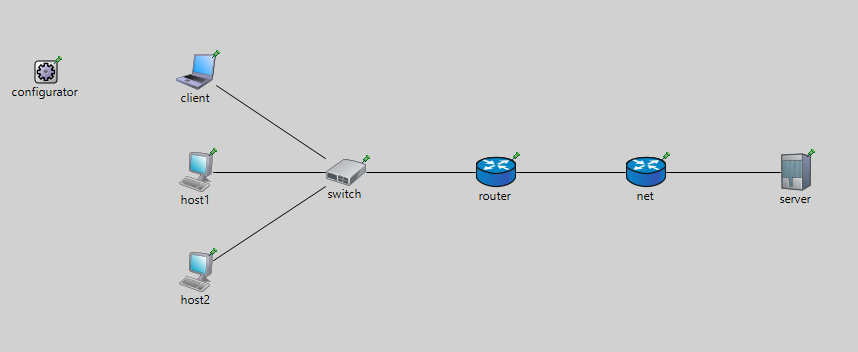
\includegraphics[width=1\textwidth]{arptest.png}
    \caption{Primer omrežja, kjer se odjemalci povežejo na strežnik preko stikal in usmerjevalnikov} 
    \label{fig:arptest}
\end{figure}

V simulaciji omrežja, definirani v datoteki $omnetpp.ini$, se odjemalec $clinet$ želi povezati na strežnik, zato pošlje ARP zahtevek v omrežje. Ta zahtevek se preko stikala $switch$ prenese na usmerjevalnik $router$, ki nanj odgovori z ARP odgovorom. Stikalo sicer zahtevek posreduje tudi napravam $host1$ in $host2$ vendar ga ti dve zavrneta. Ko odjemalec prejme ARP odgovor, pošlje SYN zahtevek strežniku, ki mu odgovori s SYN-ACK in nato še z ACK, s čimer se vzpostavi povezava med odjemalcem in strežnikom. Odjemalec nato začne pošiljati podatke strežniku, ki mu jih ta potrjuje z tcpACK.

\newpage

\subsection{vlan}

Primer prikazuje omrežje v katerem sta povezana dva odjemalca ($host1$ in $host2$) preko dveh stikal ($switch1$ in $switch2$). Vse povezave so $Eth100M$, torej ethernet povezave z kapaciteto $100Mbps$. Prisoten je tudi $configurator$, ki skrbi za dodeljevanje naslovov v omrežju.

\begin{figure}[H]
    \centering
    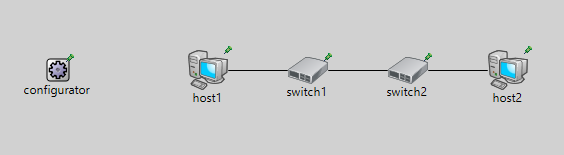
\includegraphics[width=1\textwidth]{vlan.png}
    \caption{Primer omrečja z dvema stikaloma, kjer komunicirata dva odjemalca} 
    \label{fig:vlan}
\end{figure}

V simulaciji poteka enak postopek, kot je opisan v prejšnjem primeru, torej vzpostavljanje TCP povezacve, le da se tokrat povetava vzpostavi med odjemalecema $host1$ in $host2$. V tem primeru se podatki pošiljajo preko stikal $switch1$ in $switch2$.

\newpage

\subsection{lans}

Primer $lans$ je sestavlen iz dveh omrežij $LargeNet$ in $MixedLAN$. $LargeNet$ je kompleksnejše omrežje z več strežniki, ki strežejo odjemalcem. Strežniki so povezani neposredno na stikala, ki so med seboj povezana. Na stikala se povezuejejo LAN podomrežja različnih velikosti ($SmallLAN$, $MediumLAN$, $LargeLAN$), ki so označena z oblački. V posameznih LAN podomrežjih so povezani odjemalci.

\begin{figure}[H]
    \centering
    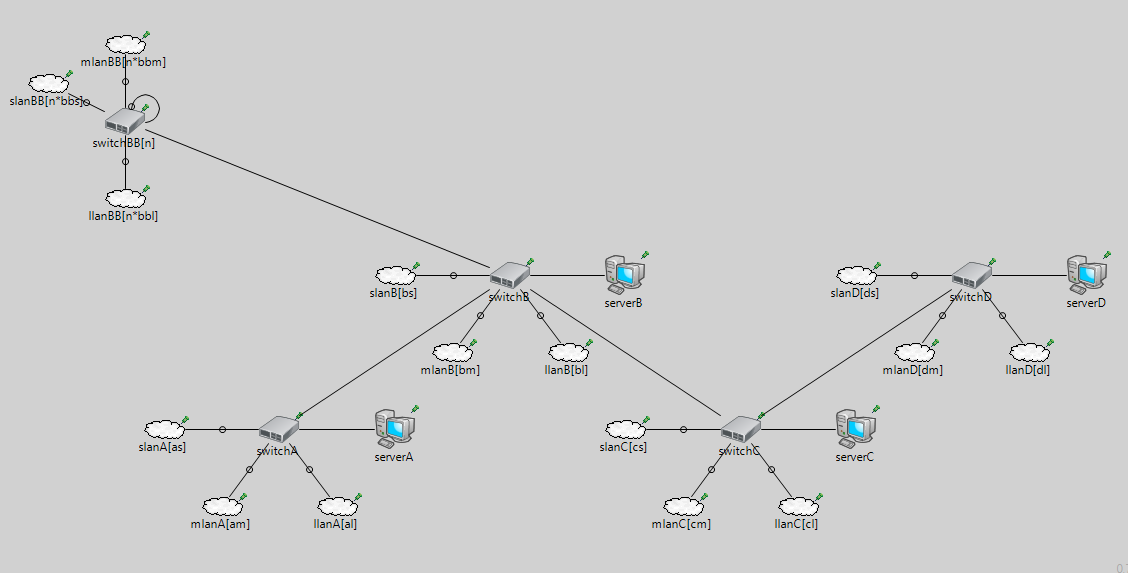
\includegraphics[width=1\textwidth]{lans-large-net.png}
    \caption{Omrežje $LargeNet$, v katerem je prek stikal povezanih več strežnikov in LAN podomrežij} 
    \label{fig:large-net}
\end{figure}

\newpage

V omrežju $MixedLAN$ pa so odjemalci na različne načine povezani na glavno vodilo ($bus$). Odjemalci $busHostA$, $busHostB$, $busHostC$ in $busHostD$ so povezani neposredno na vodilo, odjemalci $hubHostA$, $hubHostB$ in $hubHostC$ pa so povezani preko zvezdišča, ki je povezano na vodilo. Odjemalci $switchHostA$, $switchHostB$ in $switchHostC$ pa so povezani preko stikala, ki je prav tako povezano na vodilo.

\begin{figure}[H]
    \centering
    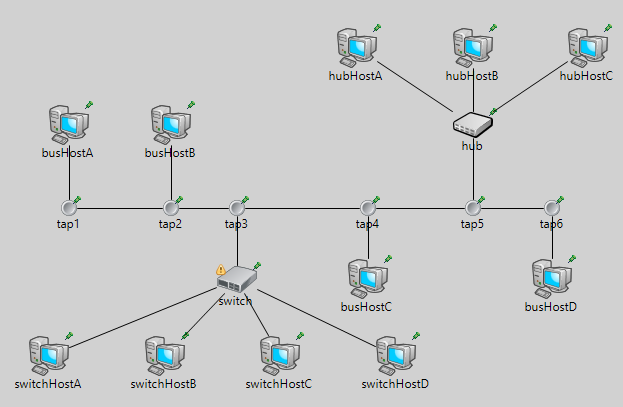
\includegraphics[width=1\textwidth]{lans-mixed-lan.png}
    \caption{LAN omrežje z različnimi načini povezovanja odjemalcev na glavno vodilo} 
    \label{fig:mixed-lan}
\end{figure}

Pri komunikaciji med odjemalci pride v omrežju do kolizij, saj se večina odjemalcev nahaja na istem vodilu, zvezdišče pa ne filtrira prometa, glede na naslovnika. Samo stikalo filtrira promet, zato med odjemalci $switchHostA$, $switchHostB$, $switchHostC$, $switchHostD$ in stikalom ne prihaja do kolizij.

\begin{figure}[H]
    \centering
    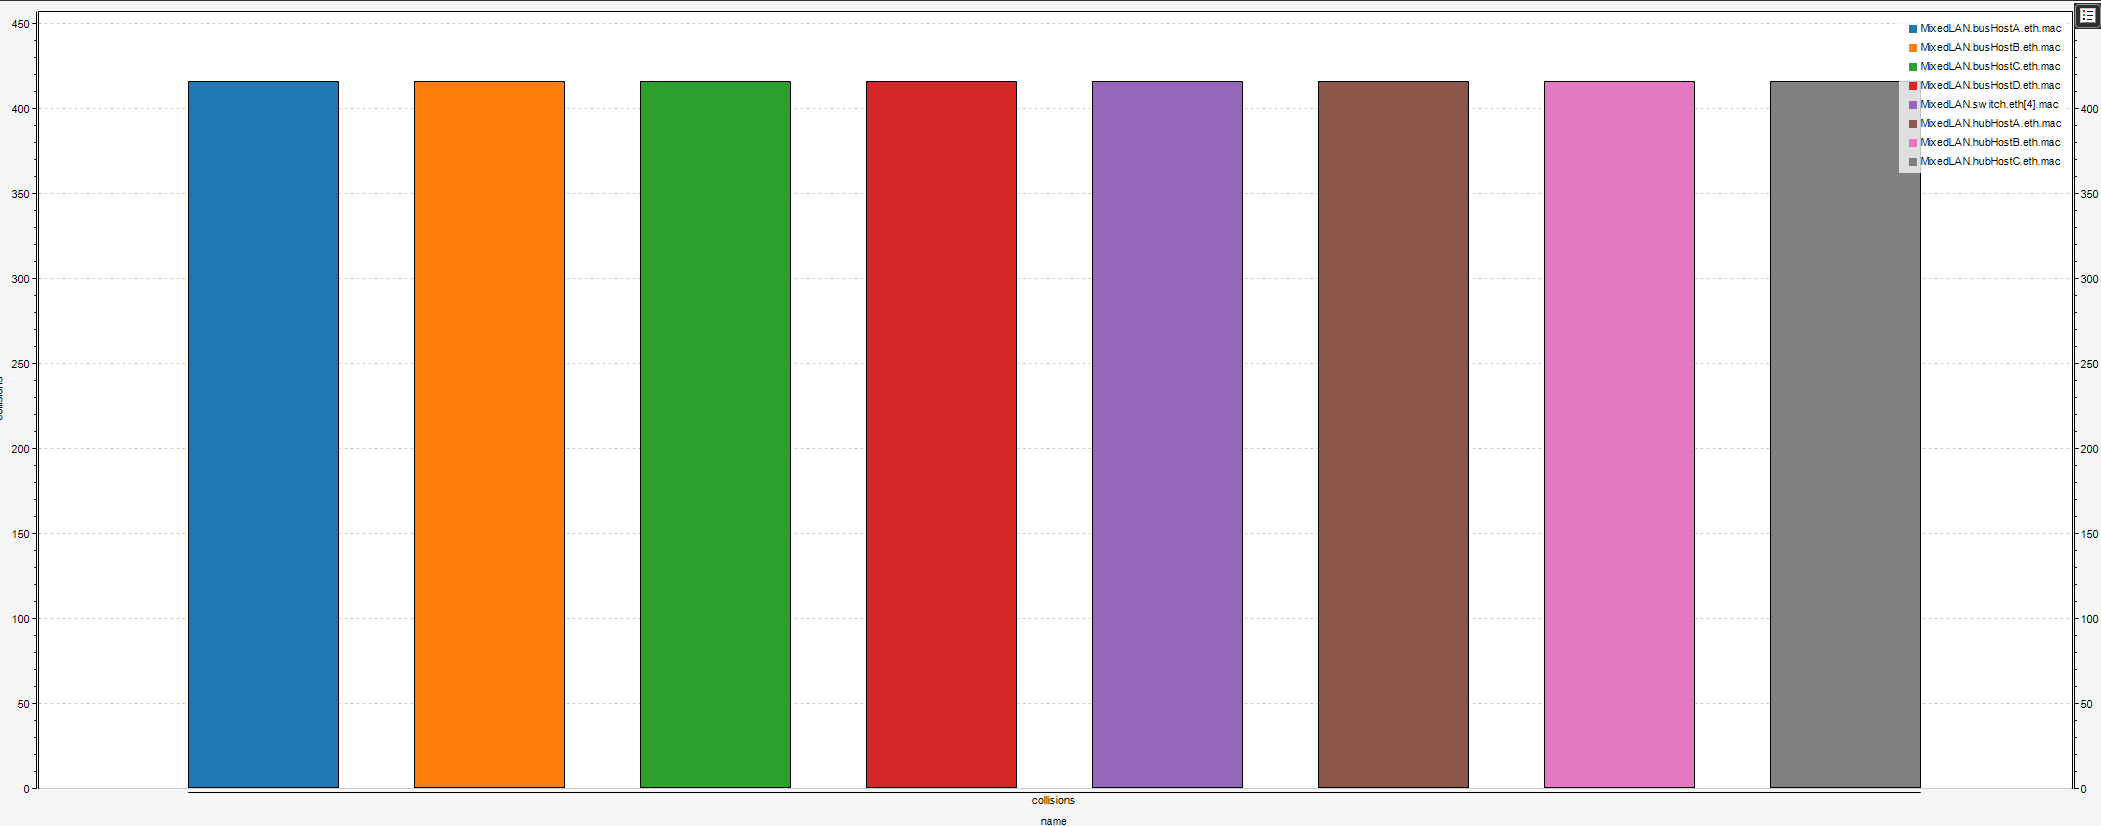
\includegraphics[width=1\textwidth]{mixed-lan-collisions-bar-chart.png}
    \caption{Število kolizij v omrežju $MixedLAN$} 
    \label{fig:mixed-lan-colisions}
\end{figure}

Posledica skupnega vodila, razvidna na sliki \ref{fig:mixed-lan-sent-recieved}, je tudi to, da vsi odjemalci prejmejo več prometa, kot ga pošljejo (razen tisti, ki generirajo promet - $switchHostA$), saj paket, poslan na vodilu pride tudi do vseh naprav, ki niso bile naslovljene in niso za stikalom.

\begin{figure}[H]
    \centering
    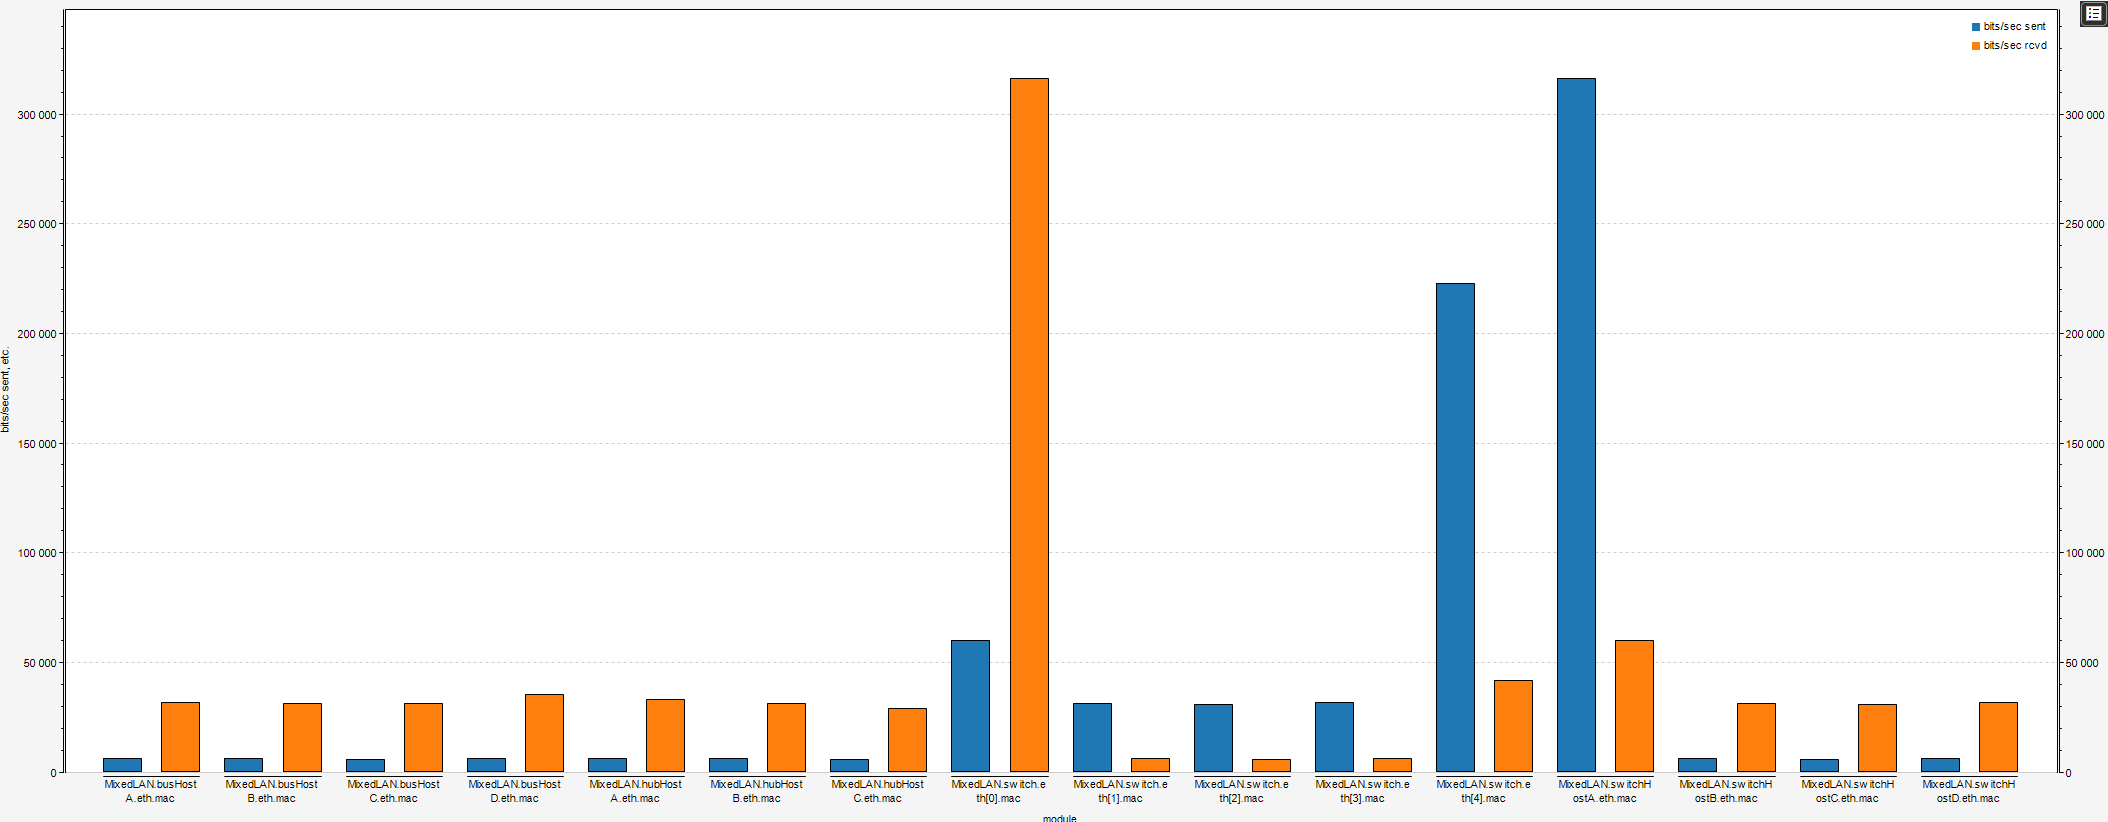
\includegraphics[width=1\textwidth]{mixed-lan-sent-recieved-bar-chart.png}
    \caption{Število poslanih in sprejetih bitov na sekundo (bps) v omrežju $MixedLAN$} 
    \label{fig:mixed-lan-sent-recieved}
\end{figure}

\section{Gradniki Ethernet omrežij}
INET ponuja številne gradnike za simulacijo Ethernet omrežij. Mnogi od teh se uporabljajo v zelo specifičnih primerih, zato jih v tem poglavju ne bomo podrobno opisali.
Kljub temu pa je nekaj gradnikov, katerih namen je bolj splošen in se jih zato da aplicirati v številnih omrežjih. Le-te bomo razdelili na dve skupini; Ethernet specifični gradniki in Splošni gradniki.
Ko omenjamo splošne gradnike se navezujemo na gradnike, ki so kompatibilni z Ethernet specifičnimi gradniki, vendar niso omejeni na uporabo le-teh.
\subsection{Ethernet specifični gradniki}
\subsubsection{Ethernet Hub}
Ethernet Hub deluje kot preprost večvratni ponavljalnik. Ko okvir prispe na katero koli izmed njegovih vrat, hub ta okvir prepošlje na vsa druga vrata. Ne pregleda in ne filtrira glede na MAC naslove. Vsaka povezana naprava vidi vsak okvir (razen na izvornih vratih).

\vspace{1em}
\noindent\begin{minipage}{\linewidth}
    \textbf{Ključne značilnosti:}
    \begin{itemize}
        \item \textbf{Oddajanje:} Vsi vhodni okviri se ponovijo na vseh vratih, kar ustvarja eno skupno domeno trkov.
        \item \textbf{Brez inteligence:} Ne izvaja učenja MAC naslovov ali upravljanja trkov.
        \item \textbf{Preprostost:} Njegovo delovanje je enostavno, modelira vedenje podobno vedenju tradicionalnih fizičnih Ethernet hubov.
    \end{itemize}

\end{minipage}

\subsubsection{Ethernet Switch}
Ethernet Switch pametno posreduje okvire med vrati na podlagi MAC naslovov. Lokacijo naprav ugotovi s pregledovanjem izvornega naslova vhodnih okvirjev in vzdržuje tabelo usmerjanja MAC naslovov. Ko okvir prispe, stikalo poišče ciljni naslov in ga pošlje samo po ustreznih vratih (če so znana) sicer pa ga odda na vsa vrata.

\vspace{1em}
\noindent\begin{minipage}{\linewidth}
    \textbf{Ključne značilnosti:}
    \begin{itemize}
        \item \textbf{Učenje MAC naslovov:} Dinamično gradi in posodablja tabelo usmerjanja za preslikavo MAC naslovov na specifična vrata.
        \item \textbf{Selektivno posredovanje:} Z zmanjšanjem nepotrebnega prometa pošilja okvire samo tam, kjer so potrebni, s čimer izolira domene trkov.
        \item \textbf{Izboljšana zmogljivost:} Z segmentacijo domen trkov stikala izboljšajo zmogljivost omrežja v primerjavi s hubi.
    \end{itemize}
\end{minipage}

\subsubsection{Ethernet Host}
Ethernet Host predstavlja končni sistem (napravo), opremljen z Ethernet vmesnikom. Vključuje Ethernet MAC (bodisi full-duplex bodisi CSMA/CD podprt), module za enkapsulacijo in omrežno plast (npr. IP, TCP/UDP) za pošiljanje in prejemanje okvirov preko žičenega medija.

\vspace{1em}

\noindent\begin{minipage}{\linewidth}
    \textbf{Ključne značilnosti:}
    \begin{itemize}
        \item \textbf{Integrirana omrežna plast:} Združuje funkcionalnosti povezovalne plasti (enkapsulacija/dekapsulacija in MAC operacije) s protokoli višje plasti.
        \item \textbf{Ethernet vmesnik:} Uporablja bodisi modul \texttt{EthernetMac} ali \texttt{EthernetCsmaMac} za prenos okvirov, odvisno od nastavitev dupleksa in upravljanja trkov.
        \item \textbf{Fizična povezava:} Povezuje se z omrežjem preko kanalov (kot je \texttt{EtherLine}), ki simulirajo fizične lastnosti Ethernet kablov.
        \item \textbf{Naslavljanje in konfiguracija:} Tipično konfiguriran z MAC in IP naslovi (bodisi statično bodisi preko omrežnih konfiguratorjev) in lahko sodeluje v komunikaciji celotnega omrežja.
    \end{itemize}
\end{minipage}

\subsubsection{Ethernet Link}
Ethernet Link modelira fizično povezavo med Ethernet napravami. Simulira lastnosti kabla, kot so zakasnitev širjenja, popuščanje signala in omejitve pasovne širine, preko katerih se prenašajo Ethernet okviri. Sam modul ne obdela okvirjev; namesto tega zagotavlja realističen kanal, ki povezuje Ethernet vmesnike.

\vspace{1em}

\noindent\begin{minipage}{\linewidth}
    \textbf{Ključne značilnosti:}
    \begin{itemize}
        \item \textbf{Fizična simulacija medija:} Zabeleži značilnosti resničnega Ethernet kabla, vključno z zakasnitvijo signala in morebitnimi izgubami.
        \item \textbf{Vedenje kanala:} Deluje kot pasivni komunikacijski kanal, ki prenaša signale med povezanimi vozlišči, ne da bi spreminjal vsebino okvirjev.
        \item \textbf{Parametrično nastavljivo:} Pogosto konfigurabilno za predstavitev različnih vrst medijev (npr. baker ali optična vlakna) z nastavitvijo lastnosti, kot so zakasnitev, stopnja bitnih napak in prenosna zmogljivost.
    \end{itemize}
\end{minipage}
\subsection{Splošni gradniki}
Opisali bomo le nekaj splošnih gradnikov, ki so vsestranski in se jih da uporabiti v številnih omrežjih. Seveda pa zdaleč ne bomo opisali vseh, saj jih je v INET-u ogromno.
\subsubsection{Wire Junction}

Wire Junction deluje kot pasivna povezovalna točka, kjer se združuje ali razhaja več ožičenih kanalov. Ne obdeluje in ne spreminja podatkovnih signalov, ki prehajajo skozi, temveč služi kot povezovalni element, ki omogoča razvejanje ali združevanje kablovskih segmentov znotraj topologije omrežja.

\vspace{1em}

\noindent\begin{minipage}{\linewidth}
    \textbf{Ključne značilnosti:}
    \begin{itemize}
        \item \textbf{Pasivni priključek:} Deluje kot fizično žično križišče, ki preprosto zagotavlja povezljivost med več kablovskimi segmenti, brez spreminjanja signala.
        \item \textbf{Fleksibilna gradnja topologije:} Omogoča ustvarjanje kompleksnih povezav, kjer je potrebno razvejanje, združevanje ali zgolj povezovanje kanalov.
        \item \textbf{Preprostost:} Zasnovan je tako, da ima minimalno vedenje; predvsem zagotavlja, da so vsi povezani kanali električno ali logično združeni, s čimer ohranja lastnosti prenesenega signala (na primer zakasnitev širjenja, ki jo določi vsak kanal).
    \end{itemize}
\end{minipage}

\subsubsection{Router}
Router deluje kot naprava za IP posredovanje, ki povezuje različna omrežja. Obdeluje pakete, ki prispejo na njegove vmesnike in na podlagi svojih usmerjevalnih tabel usmerja pakete po najbolj ustrezni poti proti njihovemu cilju.

\vspace{1em}
\noindent\begin{minipage}{\linewidth}
    \textbf{Ključne značilnosti:}
    \begin{itemize}
        \item \textbf{Posredovanje paketov:} Pregleda glavo vsakega IP paketa, da določi naslednji skok, s čimer omogoča medomrežno komunikacijo.
        \item \textbf{Usmerjevalne tabele:} Uporablja statične ali dinamične usmerjevalne protokole za gradnjo in vzdrževanje tabel, ki preslikavajo ciljna omrežja na specifične vmesnike ali naslednje skoke.
        \item \textbf{Več vmesnikov:} Običajno opremljen z več omrežnimi vmesniki, ki se lahko povezujejo z različnimi omrežnimi segmenti, kar mu omogoča premostitev ločenih oddajnih domen.
    \end{itemize}
\end{minipage}

\subsubsection{Standard host}
Standard host je obsežen simulacijski model, ki predstavlja tipični končni sistem ali računalnik. Združuje popolno omrežno plast (vključno z ravnmi, kot so IP, TCP/UDP in aplikacije) skupaj z enim ali več omrežnimi vmesniki, kar omogoča realističen posnetek obnašanja gostitelja v omrežju.

\vspace{1em}

\noindent\begin{minipage}{\linewidth}
    \textbf{Ključne značilnosti:}
    \begin{itemize}
        \item \textbf{Integrirana omrežna plast:} Združuje protokolne plasti (od fizične, povezavne do aplikacijske) za simulacijo end-to-end komunikacije, kar omogoča realističen proces paketov skozi omrežno plast.
        \item \textbf{Več vmesnikov:} Pogosto podpira enega ali več omrežnih vmesnikov (npr. Ethernet) za povezavo z različnimi omrežnimi segmenti, s čimer simulira sisteme, ki so večkrat povezani na omrežje.
        \item \textbf{Podpora za aplikacije:} Zmožen je zagnati različne aplikacijske module (odjemalce, strežnike ali druge omrežne aplikacije), ki generirajo in odgovarjajo na omrežni promet.
        \item \textbf{Konfigurabilnost:} Nudi obsežne parametre za konfiguriranje naslovov, usmerjanja, vedenja prometa in lastnosti vmesnikov, kar omogoča prilagodljivost za različne simulacijske scenarije.
        \item \textbf{Realistično obnašanje:} Odraža zakasnitve, čakanje v vrstah in procesiranje specifično za protokole, s čimer zagotavlja realističen prikaz zmogljivosti omrežnega gostitelja.
    \end{itemize}
\end{minipage}

\subsubsection{IPv4 Network Configurator}
IPv4 Network Configurator je modul, zasnovan za samodejno dodeljevanje IPv4 naslovov, konfiguracijo usmerjanja in nastavitev drugih parametrov IP-plasti po simuliranem omrežju. Odpravlja potrebo po ročni konfiguraciji posameznih gostiteljev ali usmerjevalnikov z dinamičnim razdeljevanjem informacij o naslovih glede na topologijo omrežja.

\vspace{1em}

\noindent\begin{minipage}{\linewidth}
    \textbf{Ključne značilnosti:}
    \begin{itemize}
        \item \textbf{Samodejno dodeljevanje naslovov:} Samodejno generira in dodeljuje IP naslove ter maske podomrežij vsakemu omrežnemu vmesniku v simulaciji, s čimer zagotavlja konsistentnost po celotnem omrežju.
        \item \textbf{Konfiguracija usmerjevalnih tabel:} Izračuna in namesti vnose v usmerjevalnih tabelah za vsa udeležena vozlišča, kar omogoča posredovanje paketov med različnimi podomrežji brez ročnega posega.
        \item \textbf{Zavedanje topologije:} Uporablja omrežno topologijo, definirano v simulaciji (prek NED datotek in konfiguracij), za določitev naslovnih shem in poti, ter se dinamično prilagaja spremembam, če je to potrebno.
        \item \textbf{Poenostavitev simulacij:} Poenostavi postopek namestitve v velikih ali kompleksnih simulacijah z centralizacijo in avtomatizacijo konfiguracije IP nastavitev za celotno omrežje.
    \end{itemize}
\end{minipage}

\section{Konstrukcija in analiza omrežij}

\subsection{Izbira parametrov}

Odločili smo se za naslednjih šest parametrov, za katere smo ugotavljli vpliv na delovanje omrežja:

\begin{itemize}
    \item \textbf{Interval pošiljanja:} Povprečen čas med dvema zaporednima paketoma, poslanima iz odjemalca. Čas ni konstanten, temveč je porazdeljen po eksponentni porazdelitvi.
    \item \textbf{Velikost odziva strežnika:} Velikost odziva strežnika na zahtevo odjemalca v bajtih. 
    \item \textbf{Hitrost povezav:} Hitrost povezav med napravami v omrežju.
    \item \textbf{Duplex način povezav:} Testiranje omrežij z vključenim in izključenim duplex načinom.
    \item \textbf{CSMA/CD način:} Testiranje omrežij z vključenim in izključenim CSMA zaznavanjem kolizij.
    \item \textbf{Število odjemalcev:} Število aktivnih enot v omrežju, ki generirajo promet. Ta parameter smo si izbrali tudi za simulacijo delovanja omrežij pri podpovprečni, povprečni in nadpovprečni obremenitvi.
\end{itemize}

Za določitev obremenitve omrežja smo opazovali spreminjanje zakasnitve med časom, ko je bil paket poslan iz izvora, do časa, ko je paket prišel do ponora. Ta lastnost je ponavadi za končnega uprabnika najbol relevantna.

\subsection{Razširjena dvojna zvezda}

\subsubsection{Opis omrežja}

Omrežje vsebuje dve povezani zvezdi. V središču posamezne zvezde je stikalo na katerega sta povezana po dve zvezdišči. Na vsako izmed teh dveh zvezdišč je povezanih po $h$ odjemalcev. Vse povezave med napravami so tipa $EthernetLink$ in zakasnitvijo, ki se računa po enačbi $\frac{length}{2^8}s$ \cite{omnetpp}, kjer je length dolžina povezave v metrih. Dolžina vseh povezav je $10m$. Datarate vseh povezav se streminja v $.ini$ datoteki.

\begin{figure}[H]
    \centering
    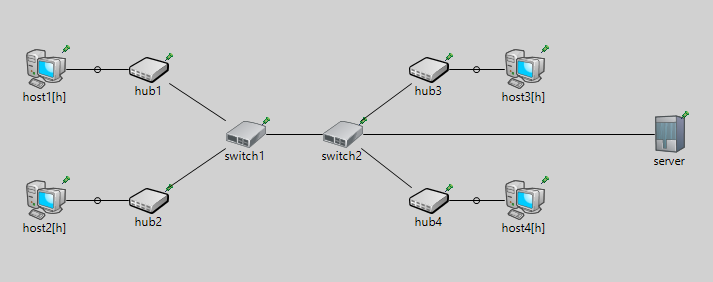
\includegraphics[width=1\textwidth]{extended-double-star/extended-double-star.png}
    \caption{Razširjena dvojna zvezda} 
    \label{fig:double-star}
\end{figure}

\subsubsection{Rezultati simulacij}

Na sliki \ref{fig:send-interval-end-to-end-delay-double-star} je prikazan vpliv intervala pošiljanja na zakasnitev paketa. Kot je razvidno iz grafa, se zakasnitev paketa povečuje z večanjem intervala pošiljanja. Vidi se mogčno spremembo pri intervalu pošiljanja okoli $0,0255s$. Za intervale večje od tega se zakasnitev zelo malo razlikuje, za intervala manjše od tega pa se zakasnitev zelo poveča. Na skrajno levi strani grafa se zdi, da se stanje spet umiri, vender je to zaradi tega, ker izgubljeni paketi ne prispevajo k zakasnitvi.

\begin{figure}[H]
    \centering
    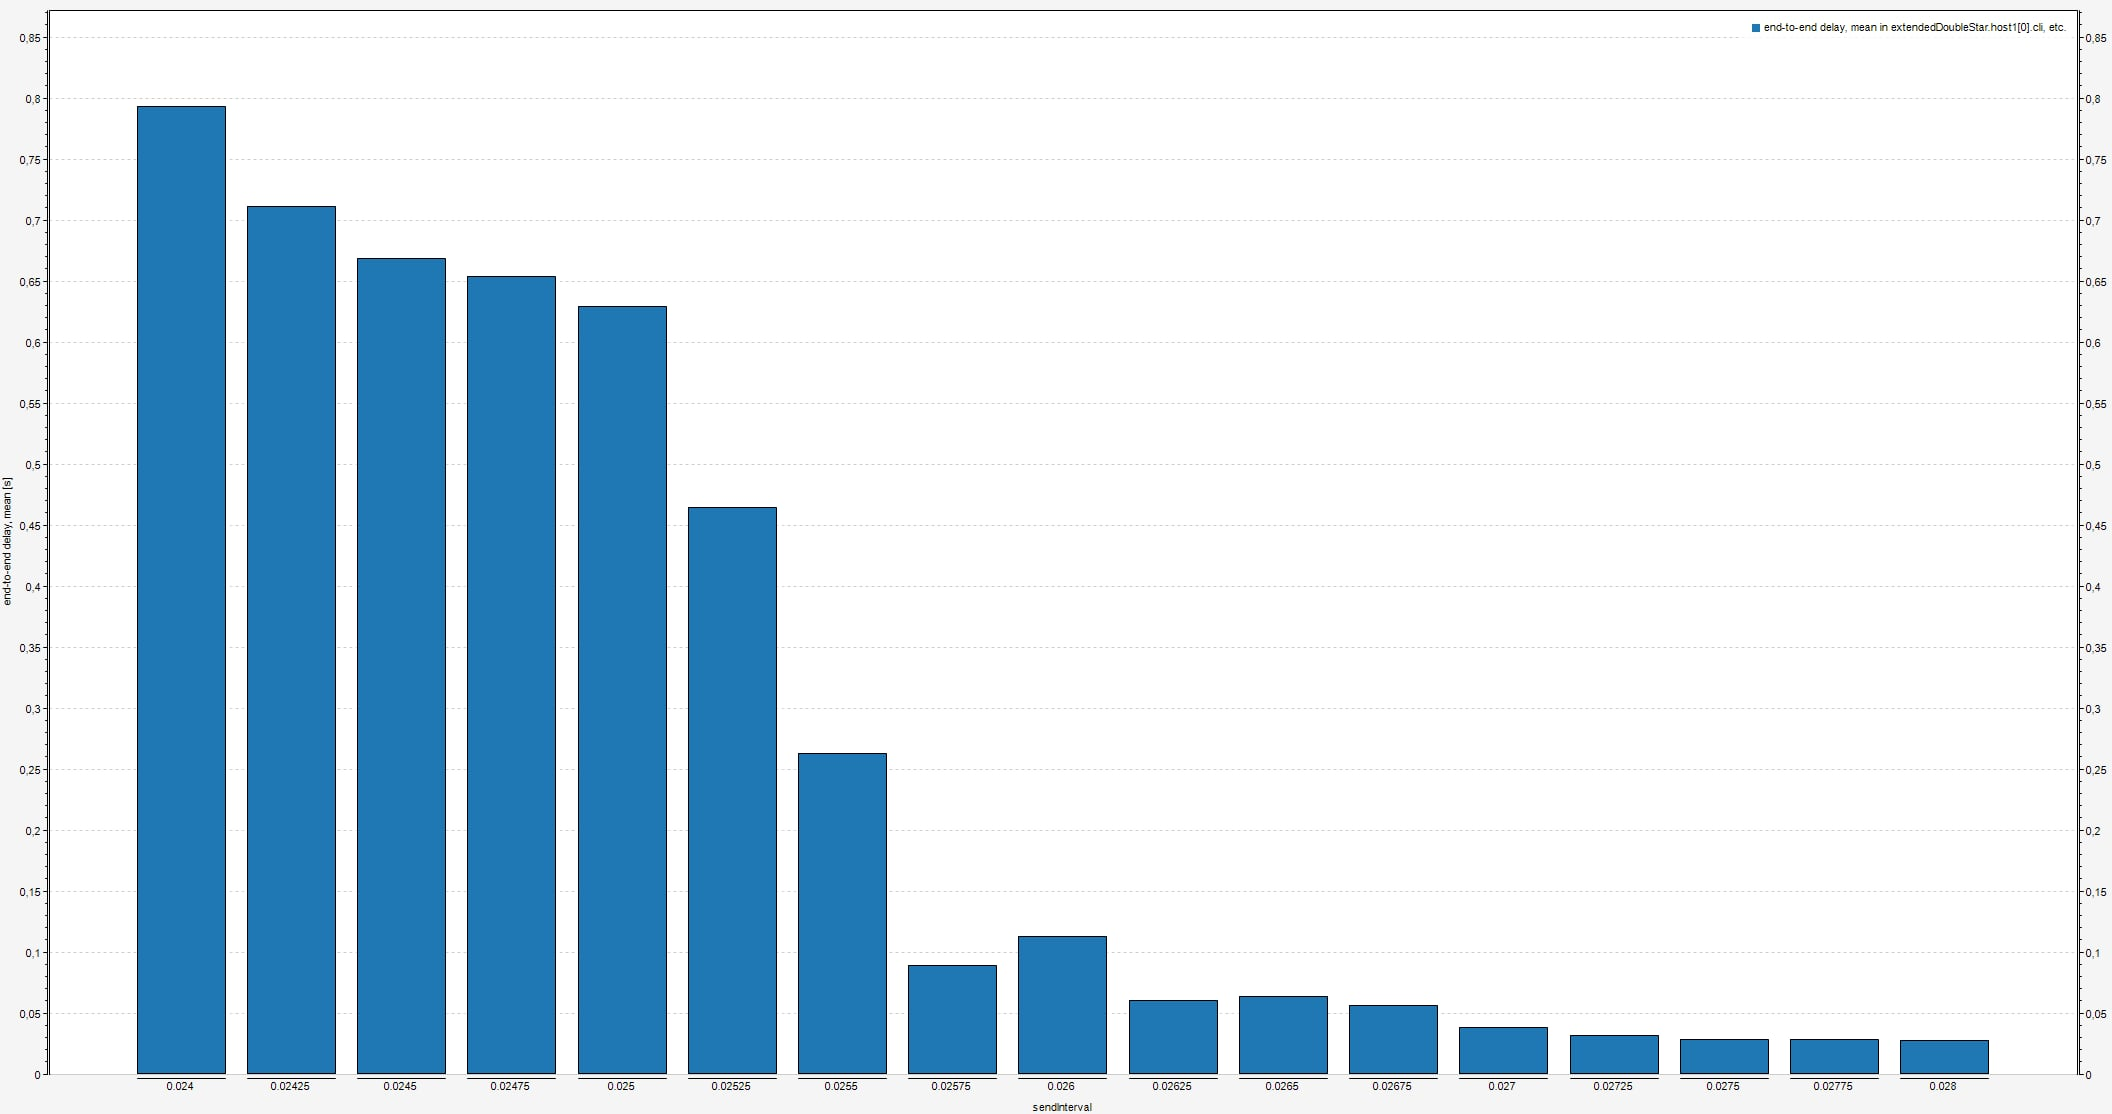
\includegraphics[width=1\textwidth]{extended-double-star/send-interval-end-to-end-delay.png}
    \caption{Vpliv intervala pošiljanja na zakasnitev paketa} 
    \label{fig:send-interval-end-to-end-delay-double-star}
\end{figure}

Zgornji graf lahko razložimo tudi z spodnjim, ki nam prikazuje povprečno zapolnjenost vrst, v odvisnosti od intervala pošiljanja. Grafa sta praktično enaka, le da je skala različna. Sklepamo lahko, da sta zakasnitev paketa linearno odvisna od zapolnjenosti vrst.

\begin{figure}[H]
    \centering
    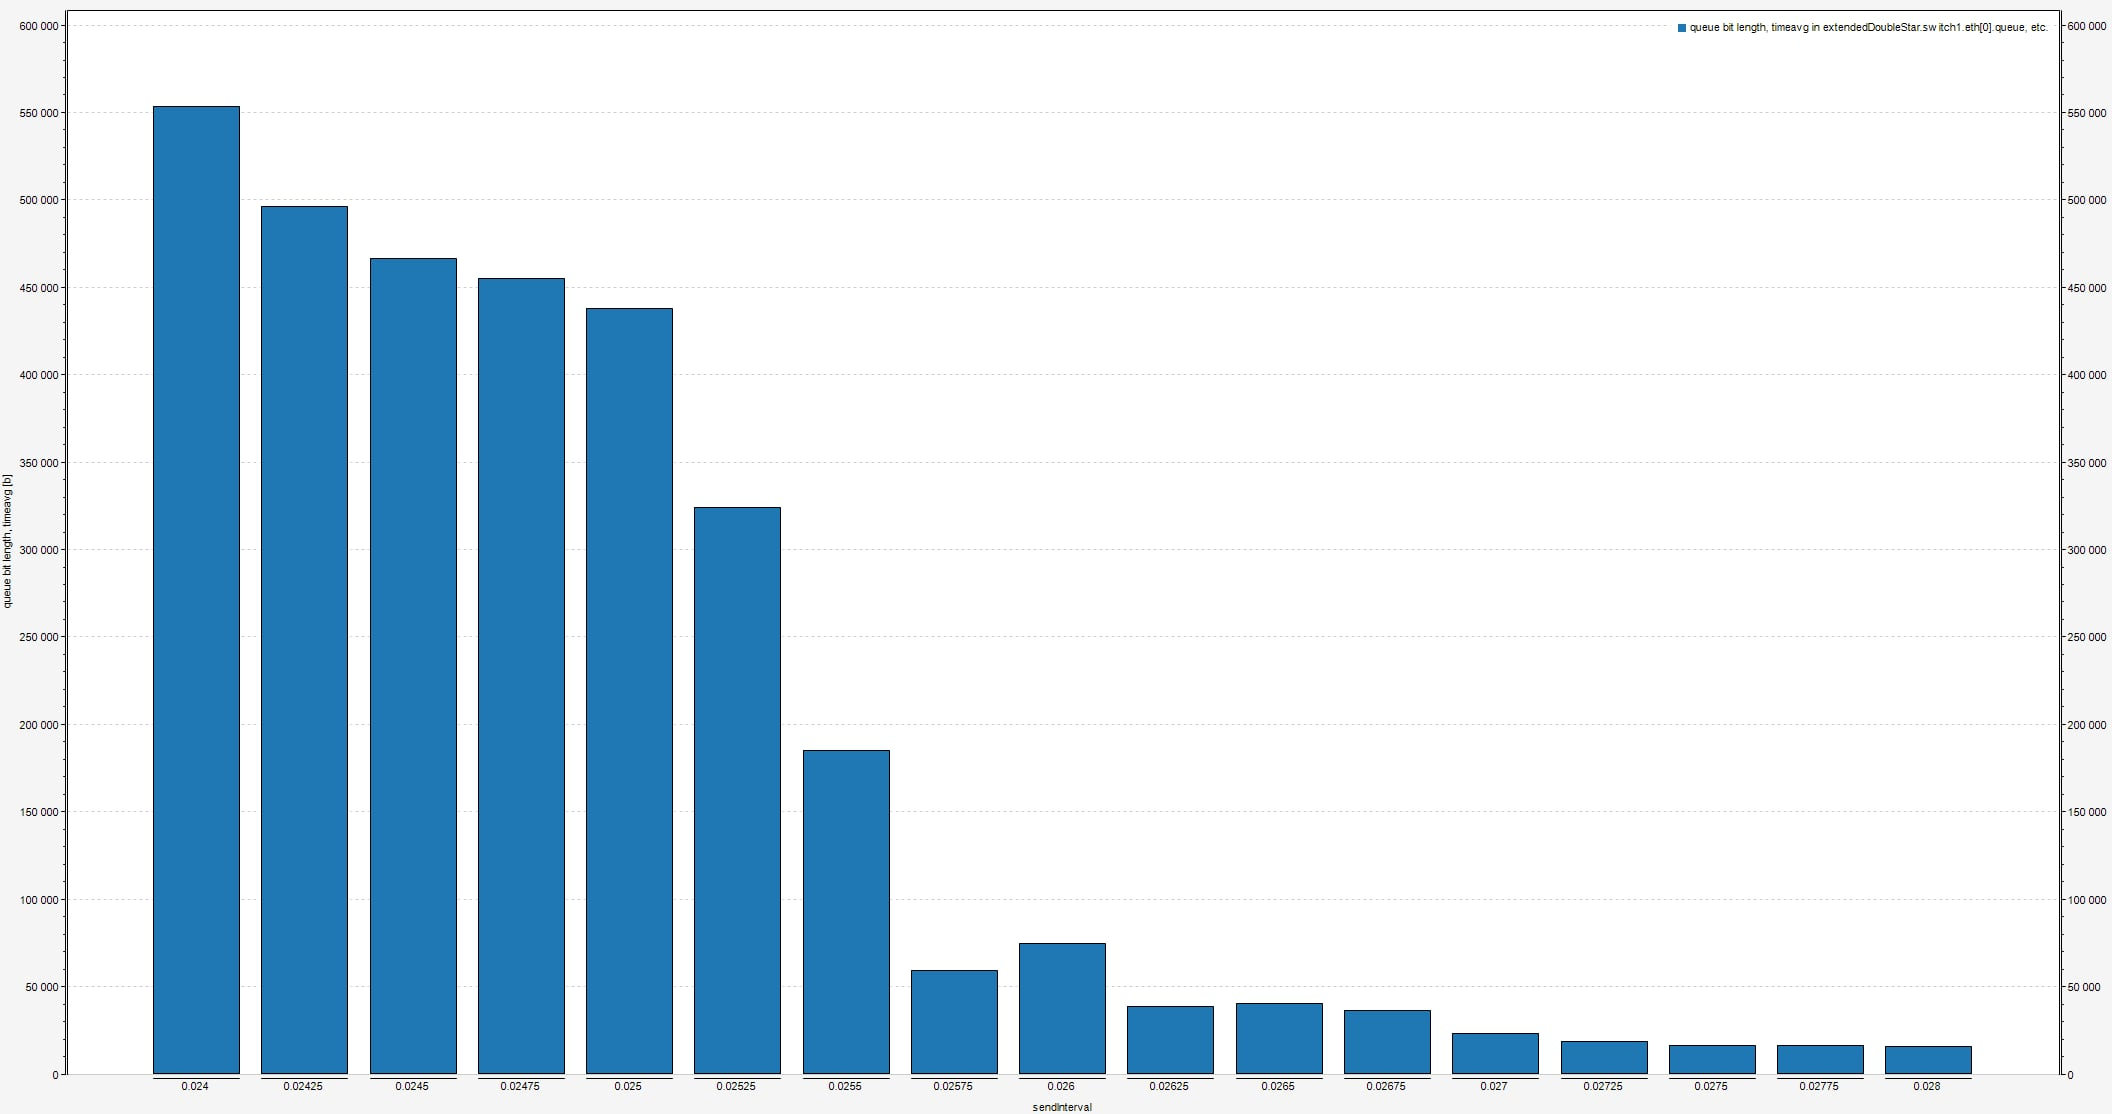
\includegraphics[width=1\textwidth]{extended-double-star/send-interval-queue-length-timeavg.jpg}
    \caption{Vpliv intervala pošiljanja na zapolnjenost čakalnih vrst} 
    \label{fig:send-interval-queue-lenght-timeavg-double-star}
\end{figure}

Naslednji graf prikazuje vpliv velikosti odziva strežnika (v bajtih) na zakasnitev paketov. Tudi tukaj je viden izjemen preskok iz sprejemlivih zakasnitev (do $0.1s$) pri velikosti odziva do $6000B$ na ogromne zakasnitve na ravni sekund pri velikosti odziva $7000B$ in več.

\begin{figure}[H]
    \centering
    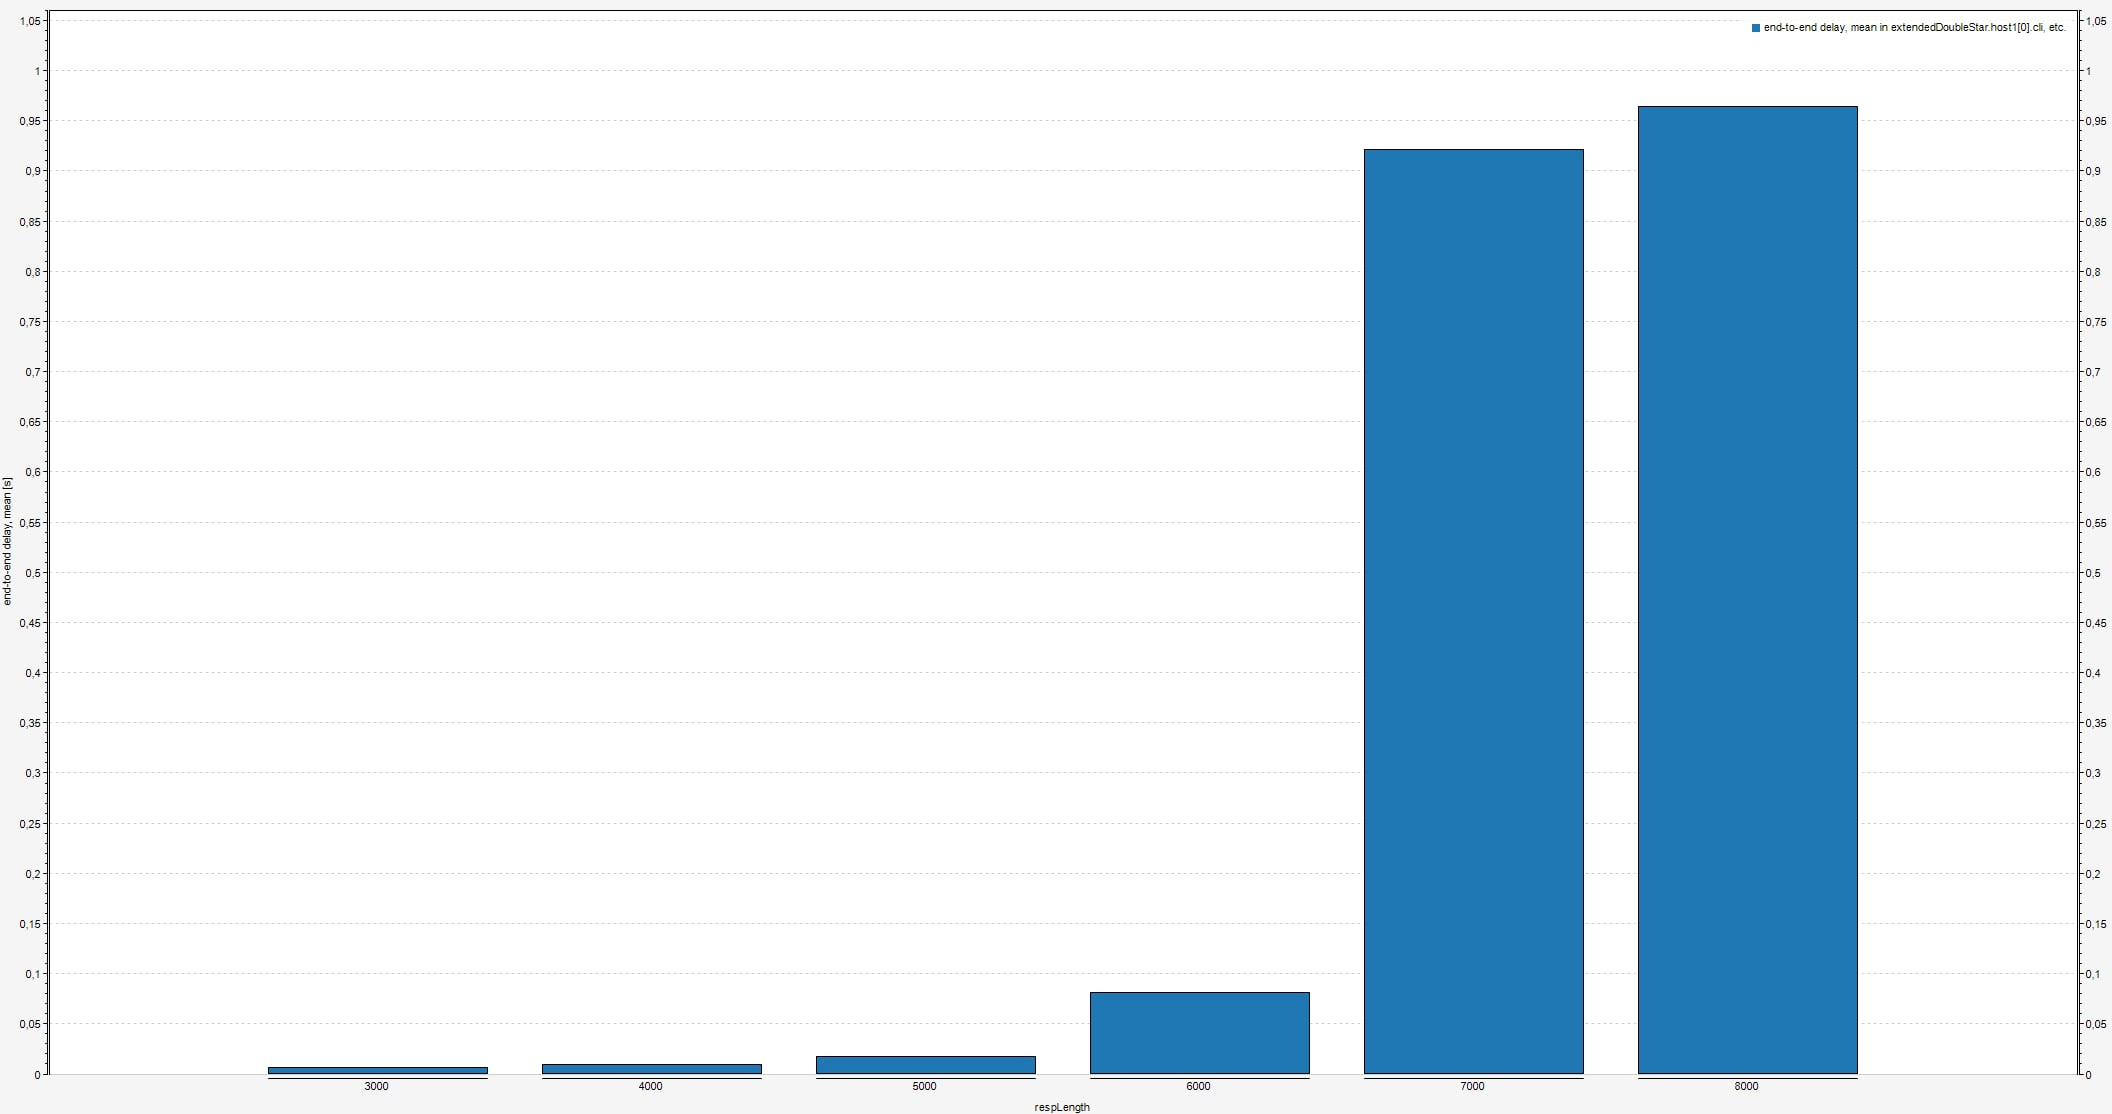
\includegraphics[width=1\textwidth]{extended-double-star/response-length-end-to-end-delay.jpg}
    \caption{Vpliv velikosti odziva strežnika na zakasnitev paketov} 
    \label{fig:response-length-end-to-end-delay-double-star}
\end{figure}

Pri naslednjem grafu je prikazan vpliv hitrosti povezav na zakasnitev paketov. Kot je razvidno iz grafa, se zakasnitev povečuje z manjšanjem hitrosti povezav. Vidi pa se tudi, da je zakasnitev v vseh primerih majhna.

\begin{figure}[H]
    \centering
    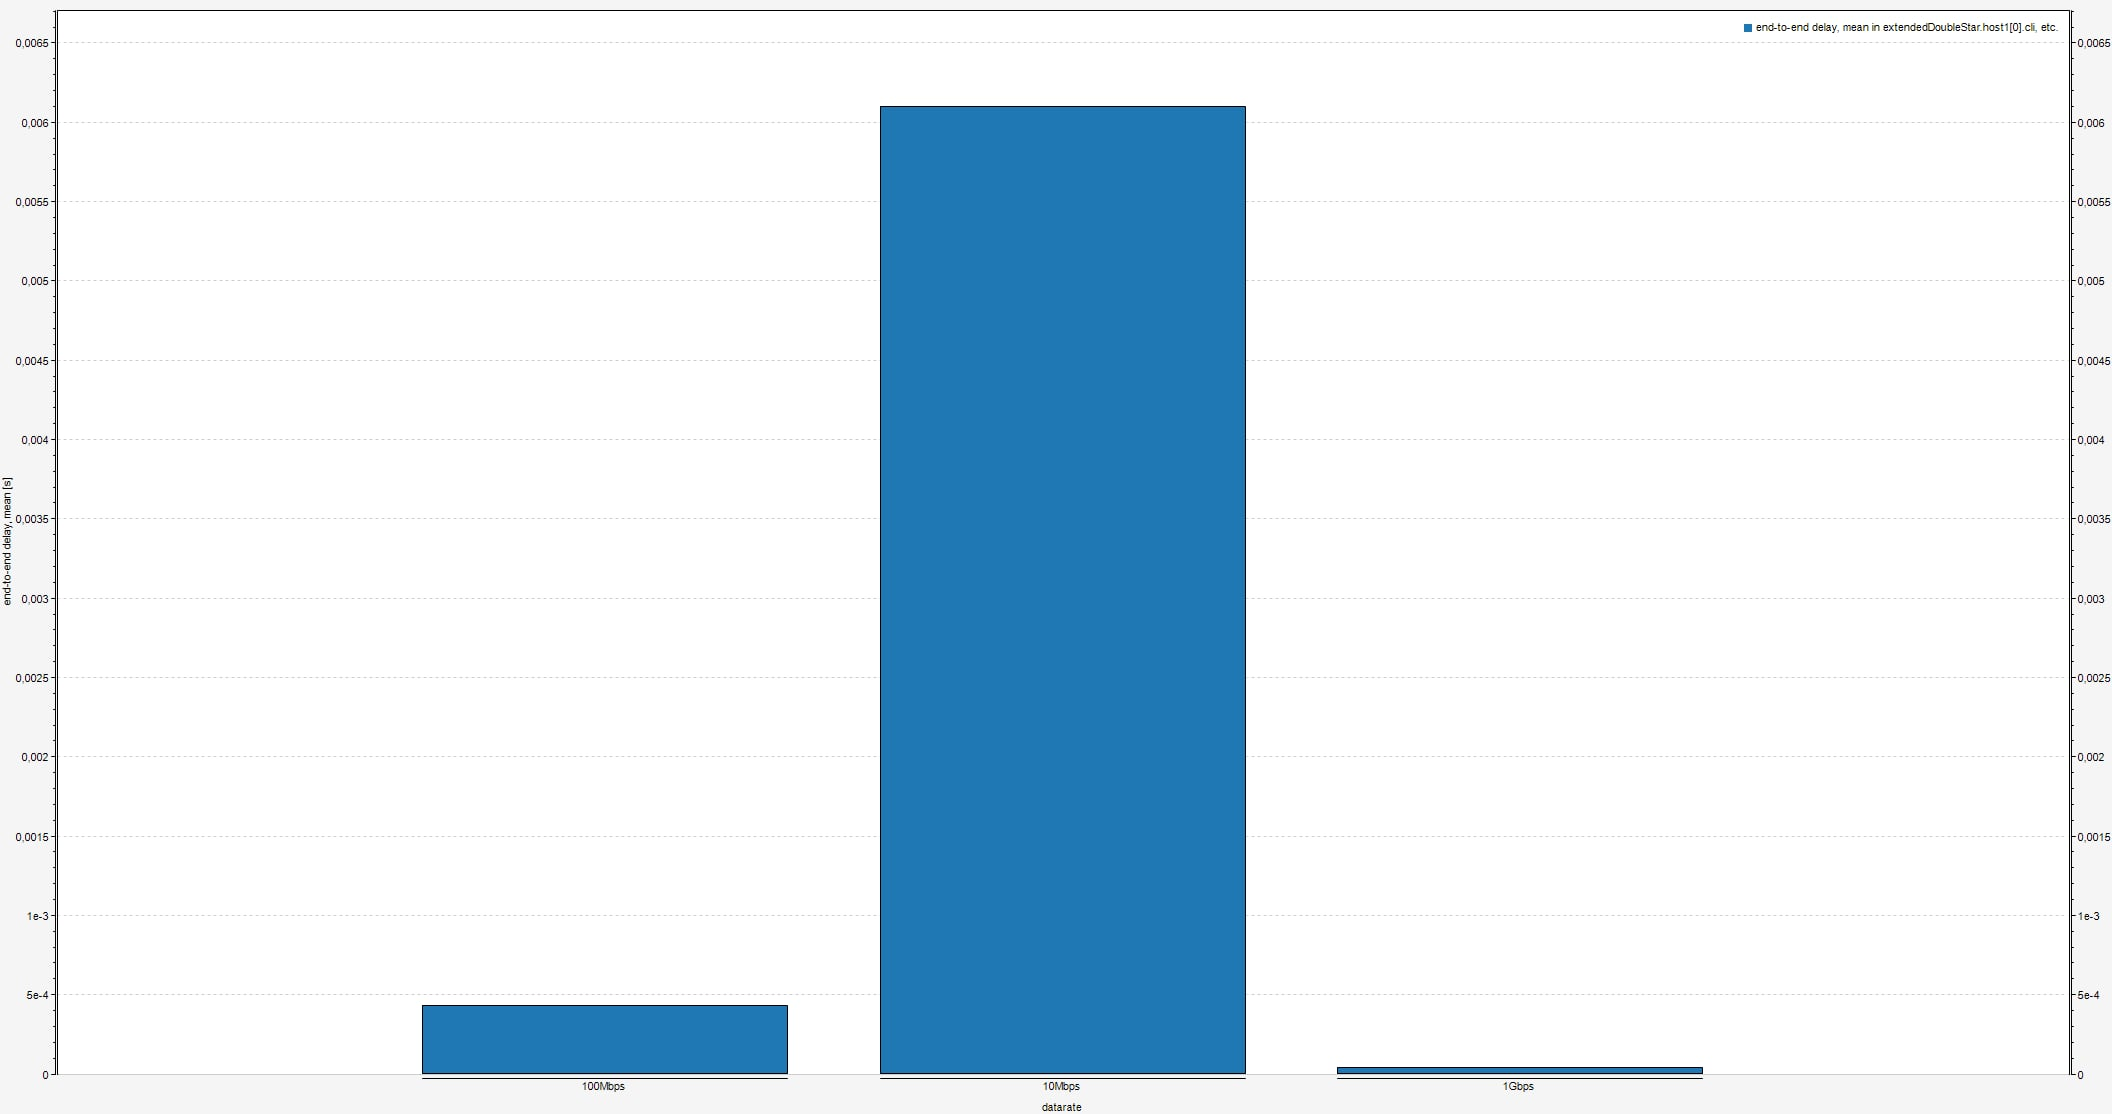
\includegraphics[width=1\textwidth]{extended-double-star/datarate-end-to-end-delay.png}
    \caption{Vpliv hitrosti povezav na zakasnitev paketov} 
    \label{fig:datarate-end-to-end-delay-double-star}
\end{figure}

Na nasledjem grafu je prikazano delovanje omrežja pri podpovprečni, povprečni in nadpovprečni obremenitvi omrežja. Razlika v zakasnitvi paketov je med podpovprečno in povprečno obremenitvijo zelo majhna, ko pa na vsak list dodamo še enega odjemalca, se omrežje nadpovprečno obremeni in zakasnitev paketov zelo poveča.

\begin{figure}[H]
    \centering
    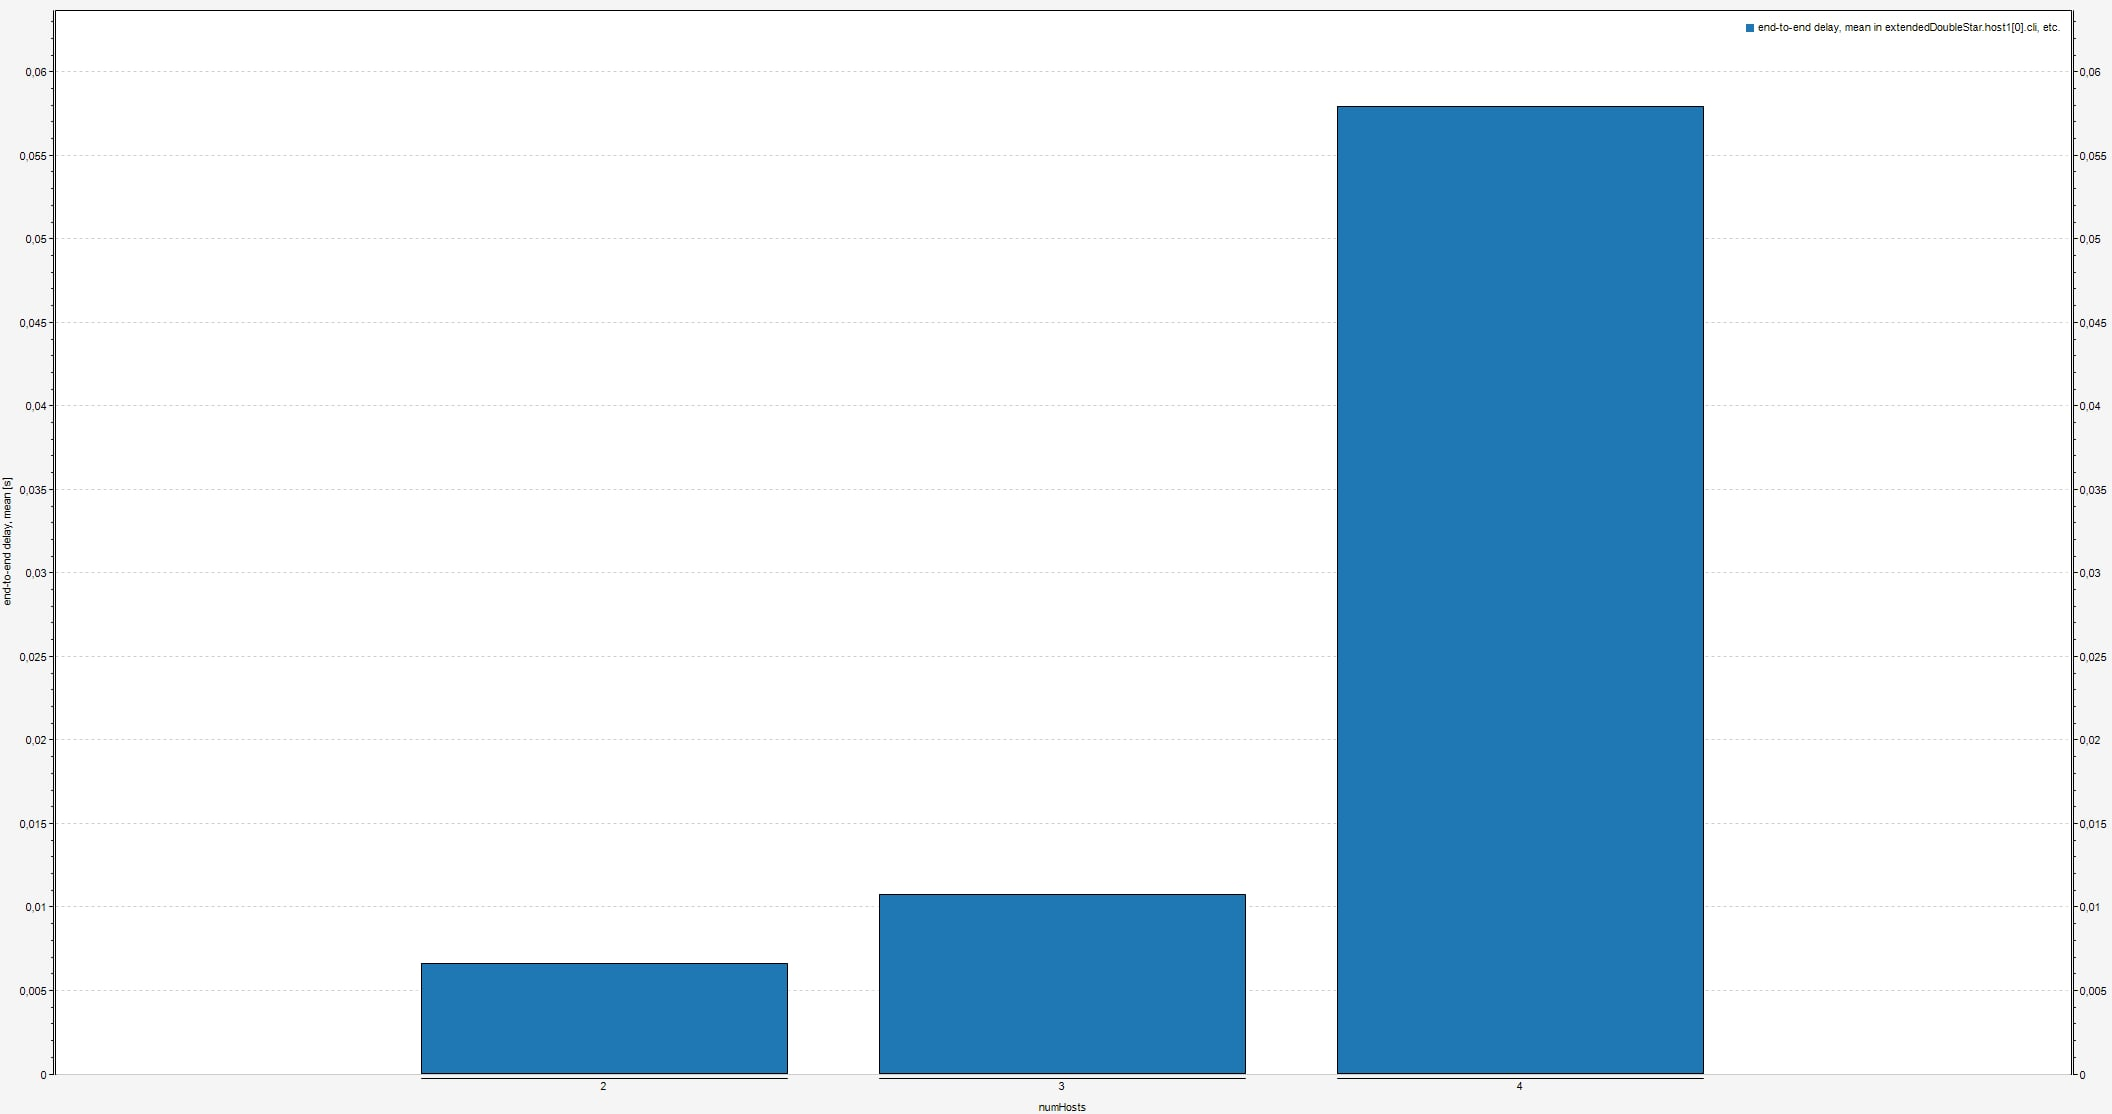
\includegraphics[width=1\textwidth]{extended-double-star/num-hosts-end-to-end-delay.png}
    \caption{Vpliv števila odjemalcev na zakasnitev paketov} 
    \label{fig:num-hosts-end-to-end-delay-double-star}
\end{figure}

\subsection{Binarno ethernet drevo}

\subsubsection{Opis omrežja}

Prikazano omrežje ima strukturo binarnega drevesa. V korenu drevesa je strežnik, nanj pošiljajo zahteve odjemalci, ki so v listih drevesa. Strežnik je z odjemalci povezan preko dveh nivojev stikal in enega nivoja zvezdišč. Vse povezave so tipa $EthernetLink$ in zakasnitvijo, ki se računa po enačbi $\frac{length}{2^8}s$ \cite{omnetpp}, kjer je length dolžina povezave v metrih. Dolžina vseh povezav je $10m$. Datarate vseh povezav se streminja v $.ini$ datoteki.

\begin{figure}[H]
    \centering
    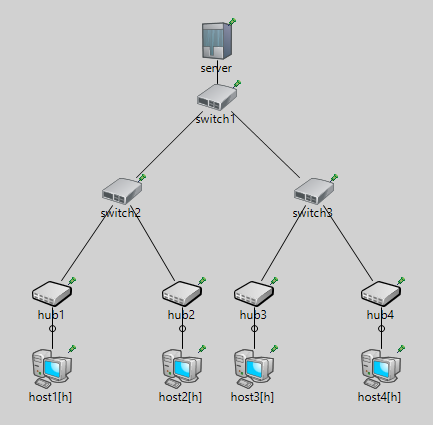
\includegraphics[width=1\textwidth]{binary-tree/binary-tree.png}
    \caption{Ethernet drevo na vodilu}
    \label{fig:eth-tree}
\end{figure}

\subsubsection{Rezultati simulacij}

Spet je opazno, skoraj enako kot pri prejšnjem omrežju, da je zakasnitev paketov močno odvisna od intervala pošiljanja paketov, z strmim dvigom pri intervalu pošiljanja okoli $0.255s$.

\begin{figure}[H]
    \centering
    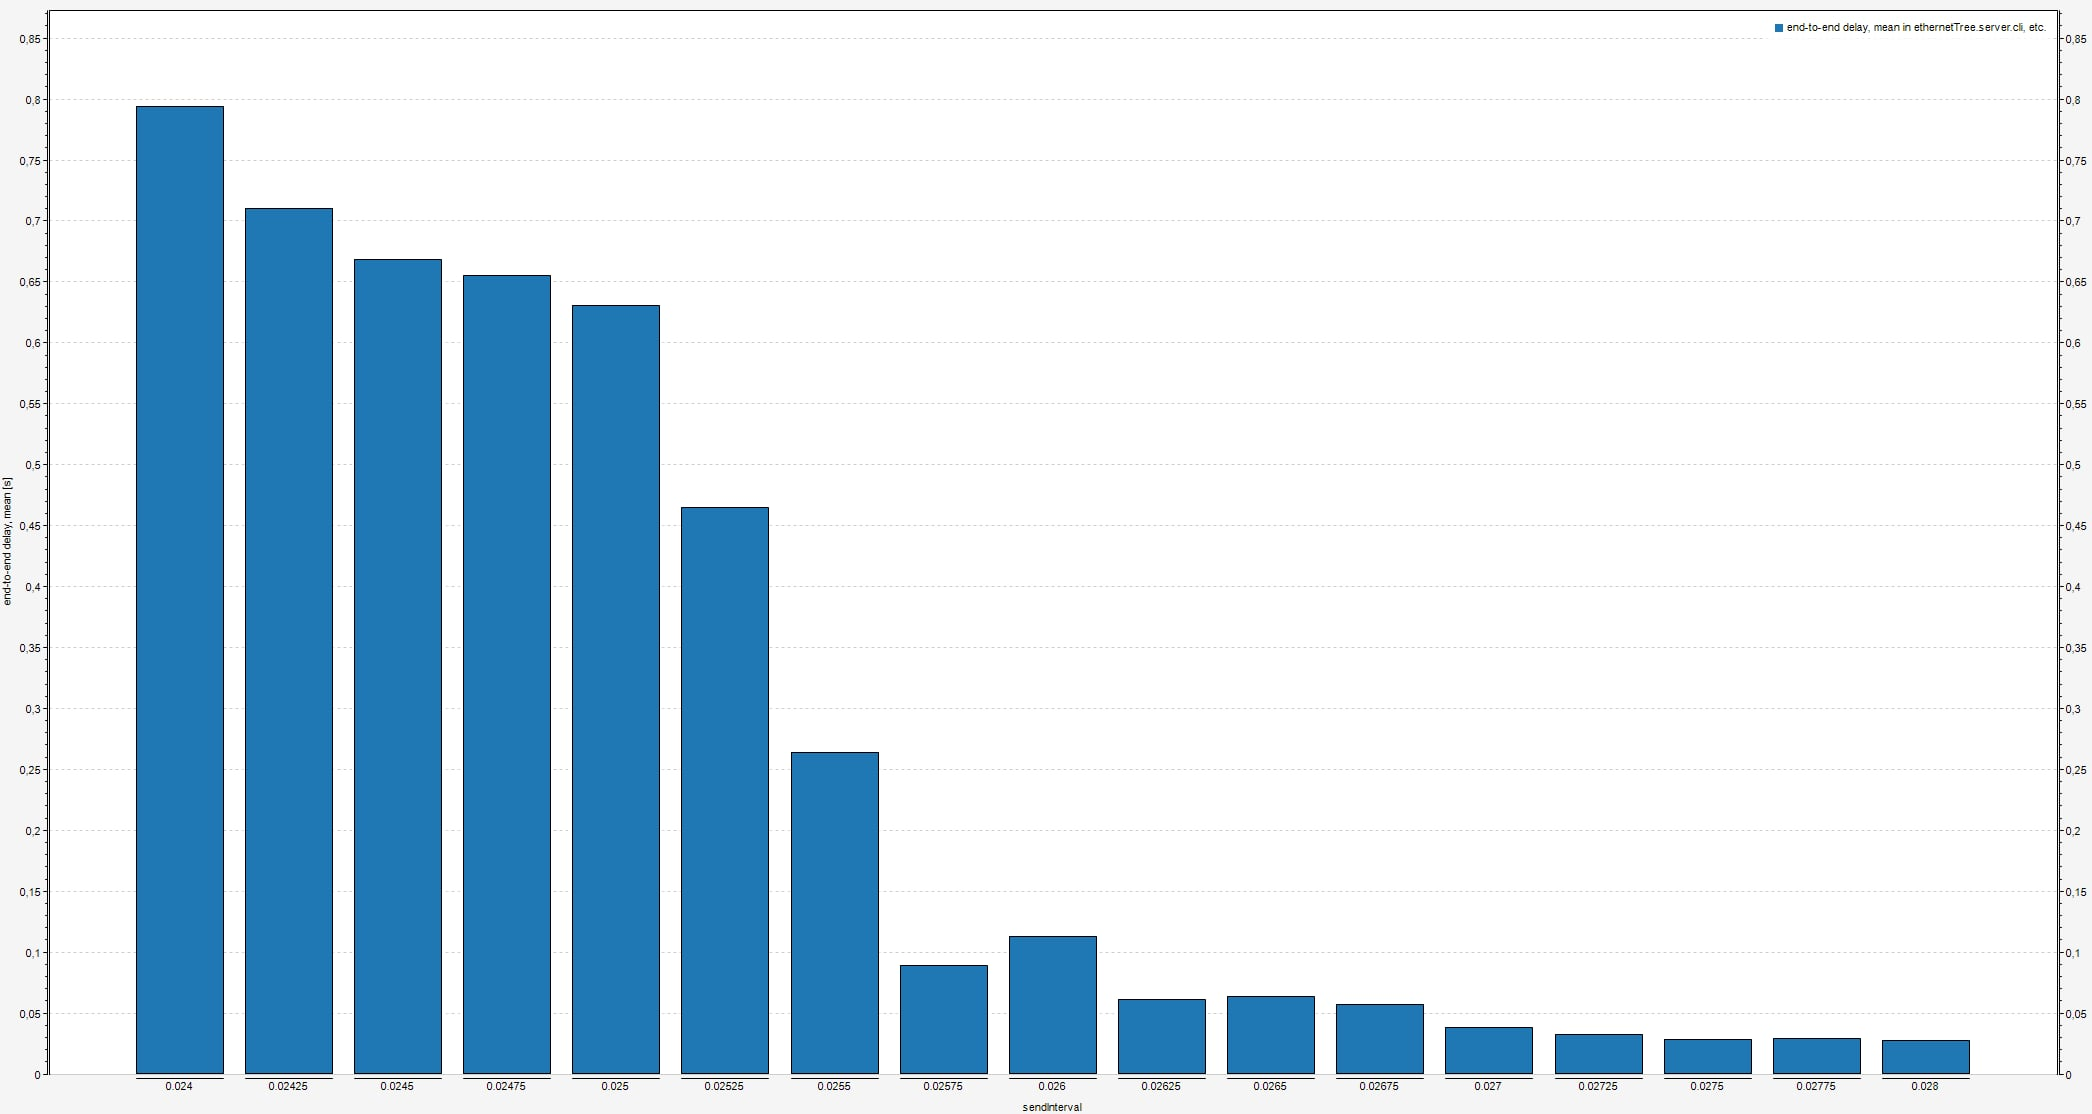
\includegraphics[width=1\textwidth]{binary-tree/send-interval-end-to-end-delay.jpg}
    \caption{Zakasnitev paketov v odvisnosti od intervala pošiljanja}
    \label{fig:send-interval-end-to-end-delay-binary-tree}
\end{figure}

Tudi v tem omrežju se zakasnitev paketov drastično poveča pri povečanju velikosti odziva strežnika iz $6000B$ na $7000B$ in več.

\begin{figure}[H]
    \centering
    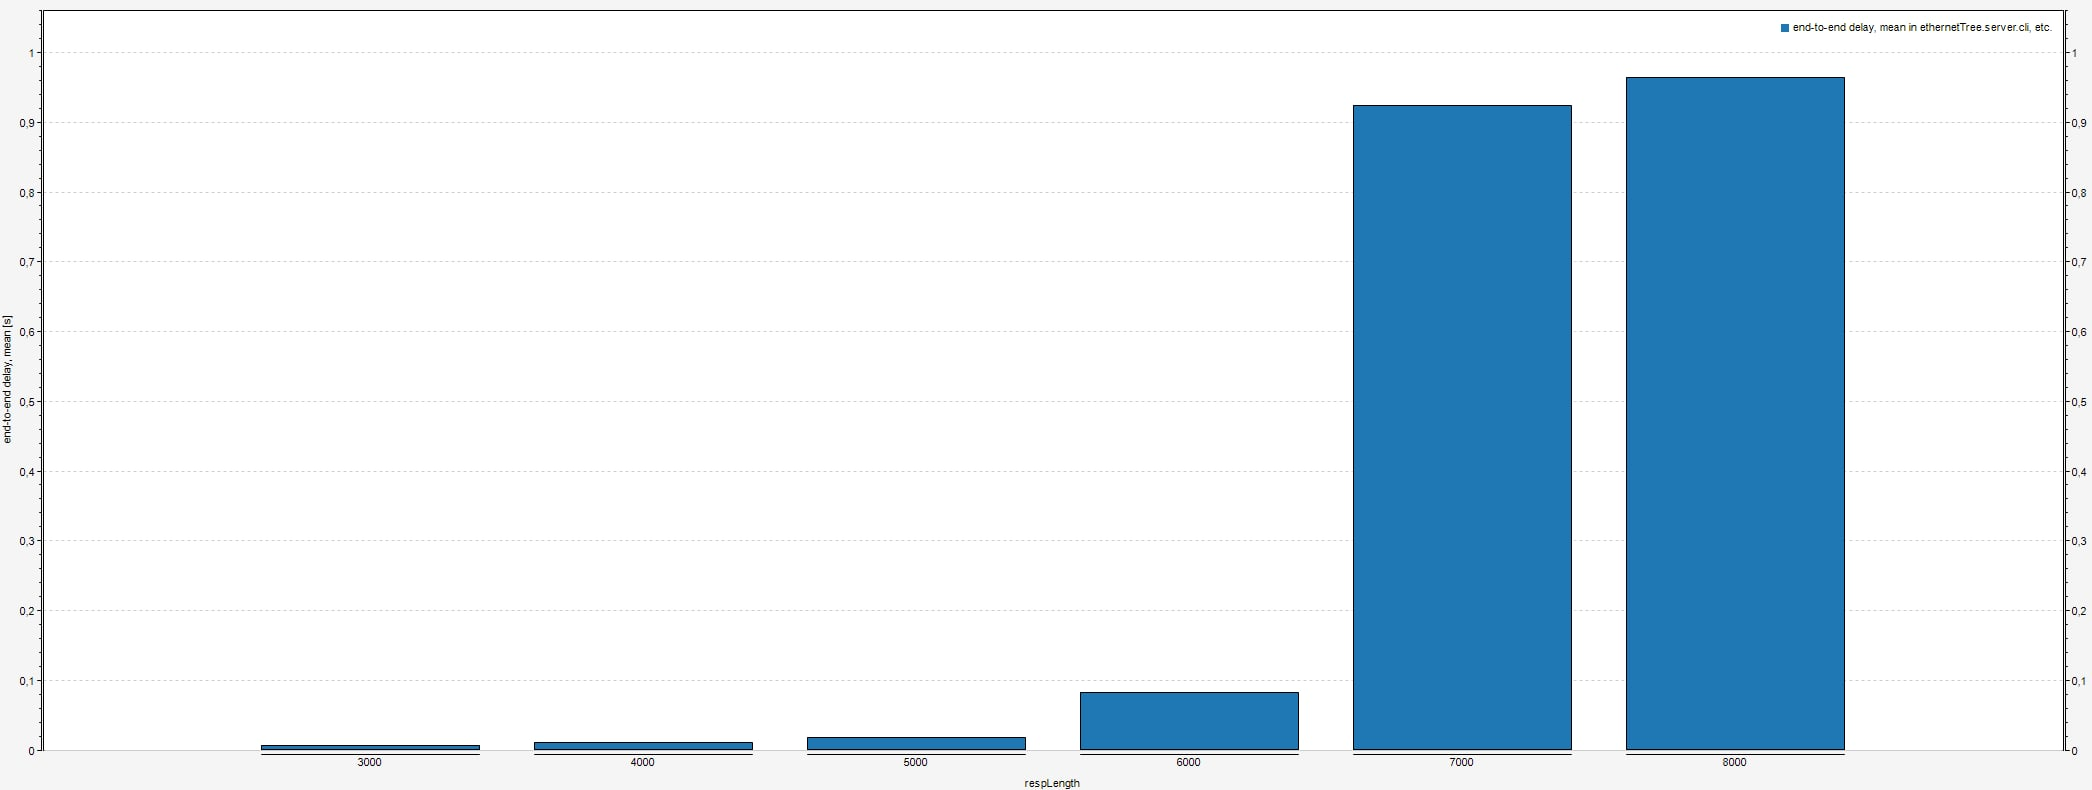
\includegraphics[width=1\textwidth]{binary-tree/response-length-end-to-end-delay.jpg}
    \caption{Zakasnitev paketov v odvisnosti od velikosti odziva strežnika}
    \label{fig:response-length-end-to-end-delay-binary-tree}
\end{figure}

Enako velja za hitrost povezav, kjer se zakasnitev povečuje z manjšanjem hitrosti povezav.

\begin{figure}[H]
    \centering
    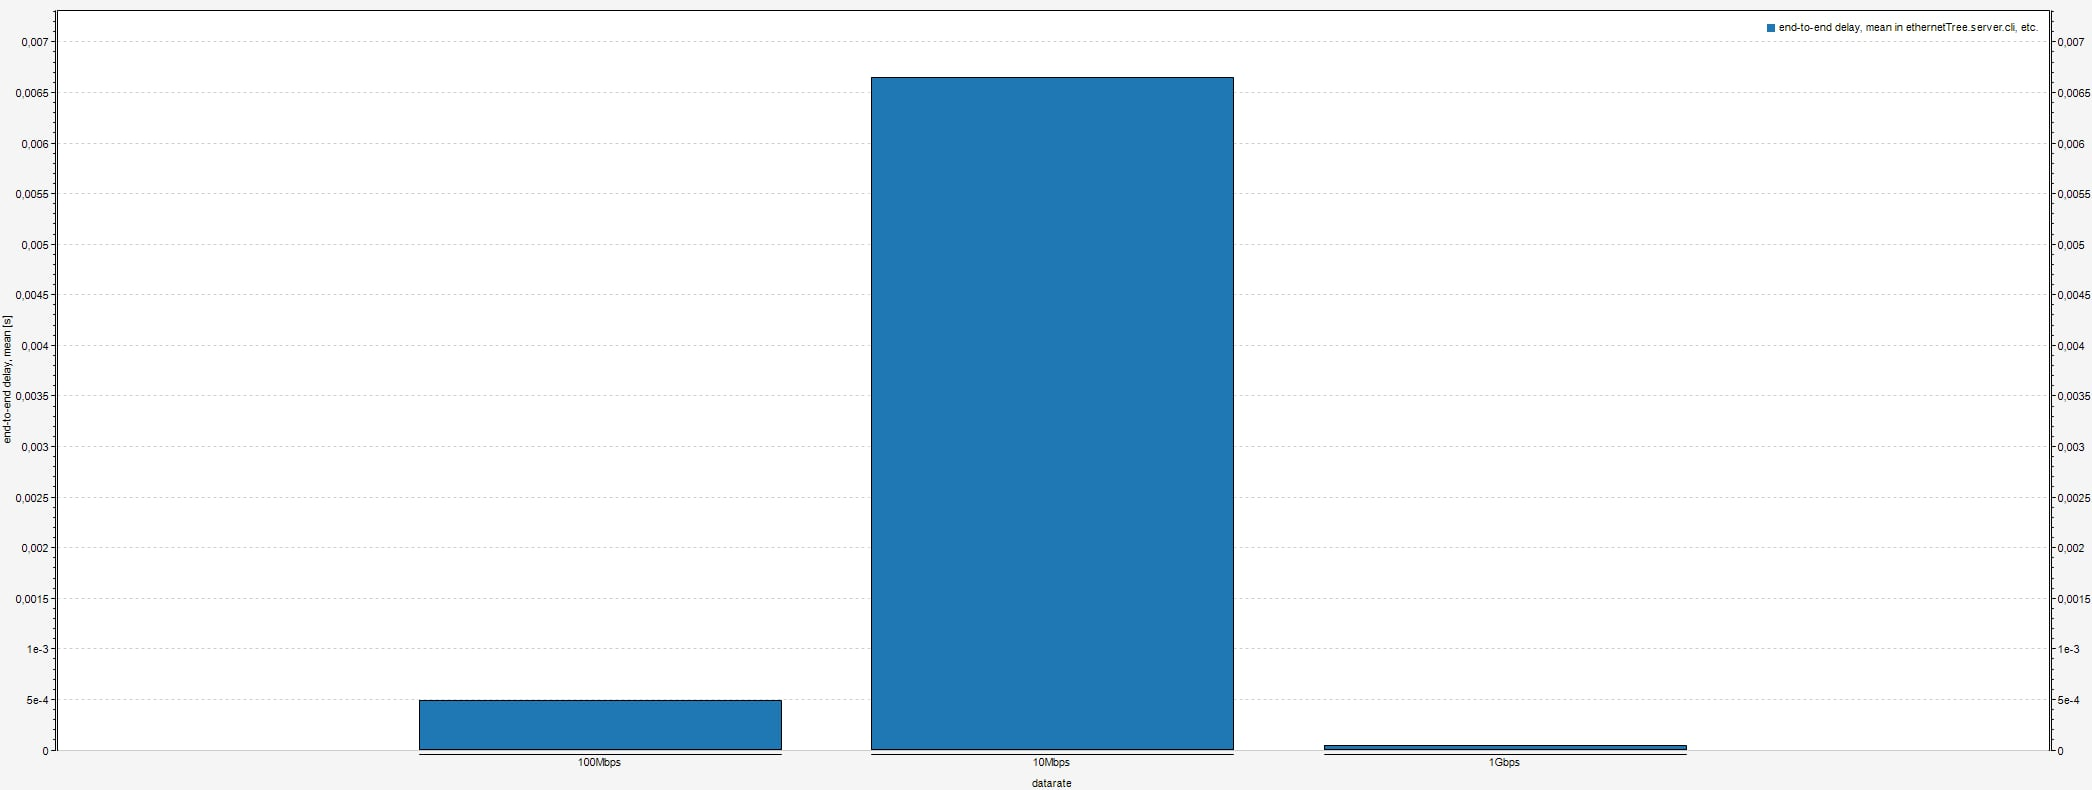
\includegraphics[width=1\textwidth]{binary-tree/datarate-end-to-end-delay.jpg}
    \caption{Zakasnitev paketov v odvisnosti od hitrosti povezav}
    \label{fig:datarate-end-to-end-delay-binary-tree}
\end{figure}

Če pogledamo zakasnitev paketov pri različnih obremenjenostih omrežja, tj. različnem številu aktivnih odjemalec spet vidimo velik preskok, ko preidemo iz povprečne obremenitve v nadpovprečno obremenitev.

\begin{figure}[H]
    \centering
    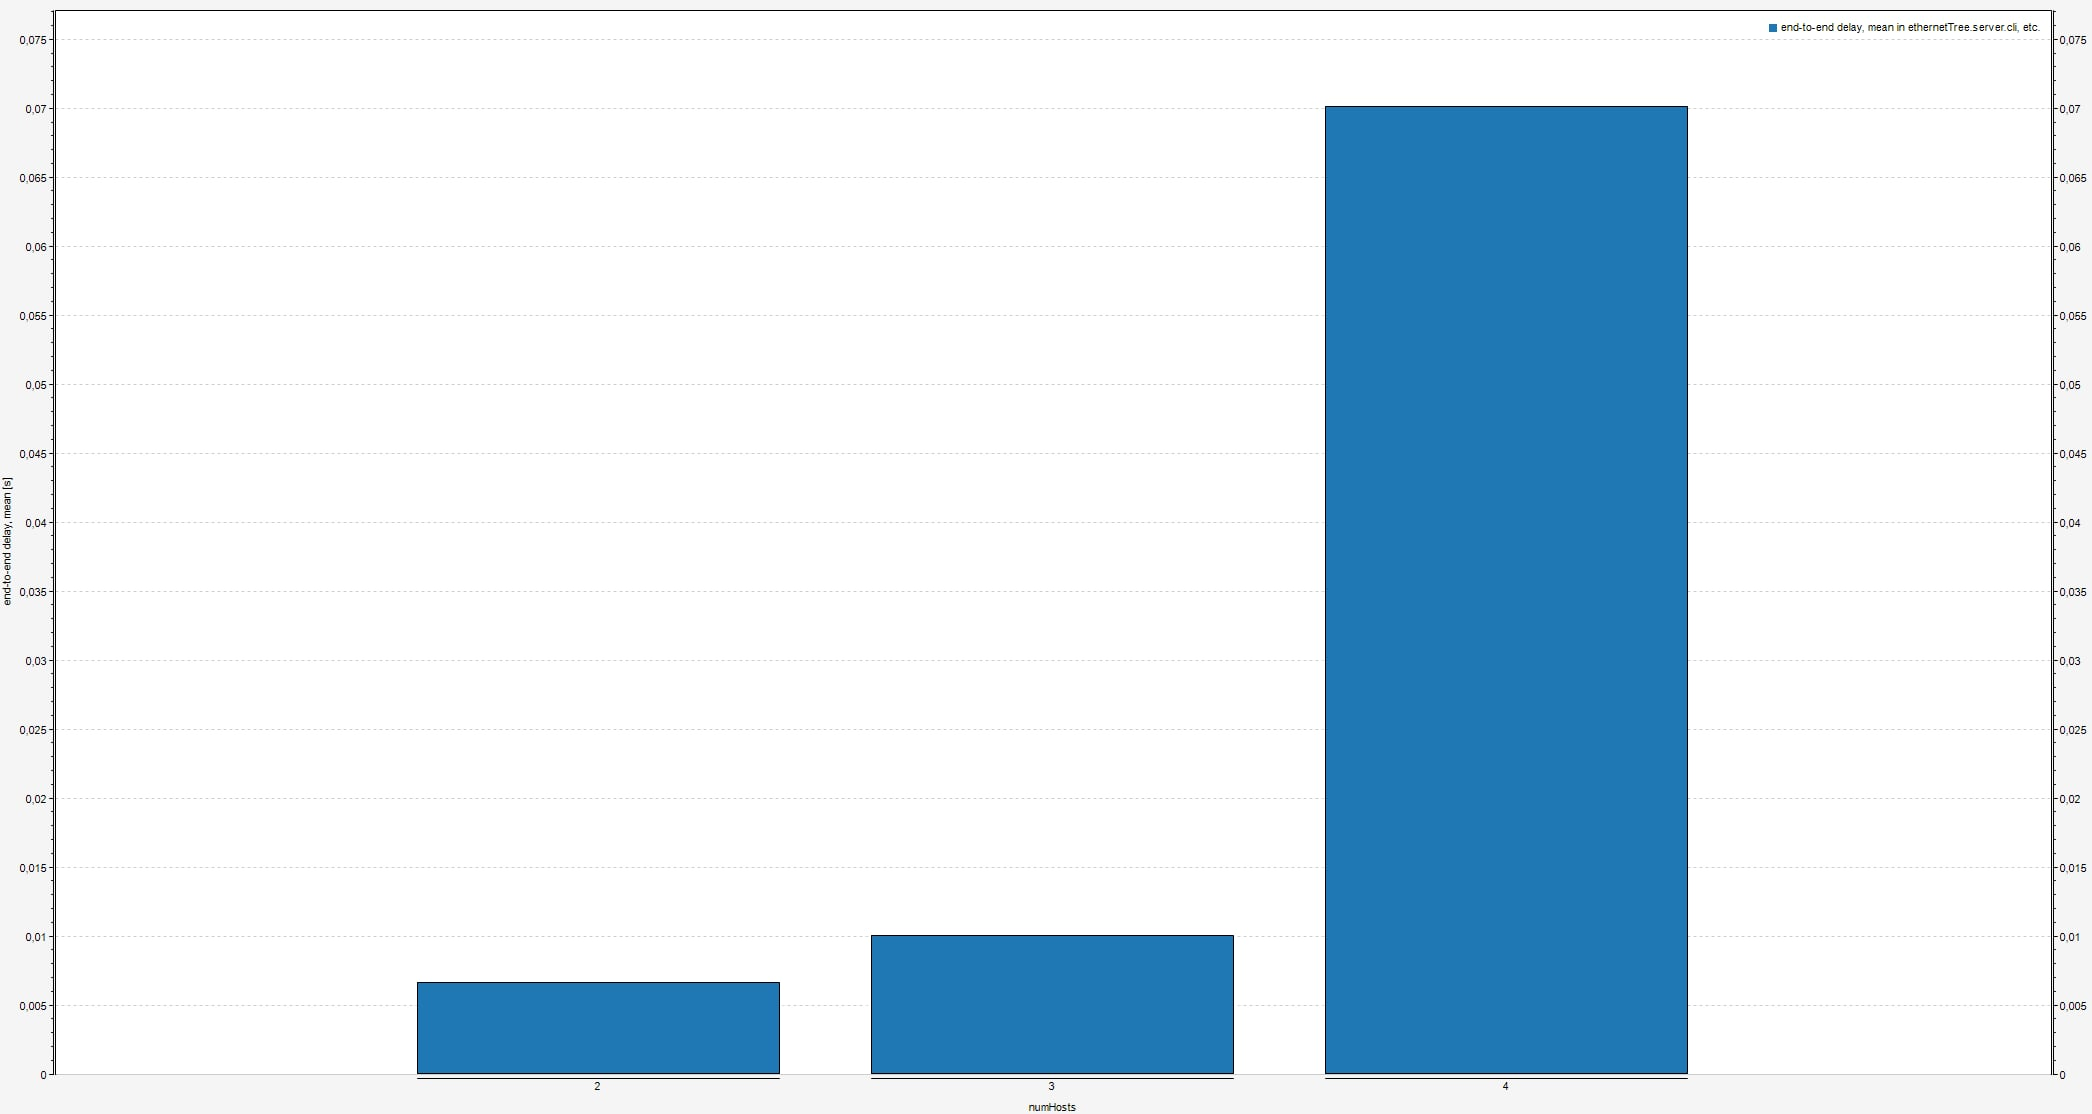
\includegraphics[width=1\textwidth]{binary-tree/num-hosts-end-to-end-delay.jpg}
    \caption{Zakasnitev paketov v odvisnosti od števila odjemalcev}
    \label{fig:num-hosts-end-to-end-delay-binary-tree}
\end{figure}

\subsection{Zaporedno vezano omrežje}

\subsubsection{Opis omrežja}
Zaporedno vezano omrežje modelira preprosto verižno topologijo ethernetnih vozlišč. Na levem koncu je en sam \texttt{EthernetHost}, ki predstavlja strežnik. Nato sledi \texttt{n} zaporedno vezanih sestavljenih modulov \texttt{HostElement}. Vsak \texttt{HostElement} vsebuje \texttt{EthernetHost} in \texttt{EthernetSwitch}.

\texttt{HostElementi} se povezujejo tako: strežnik se poveže z levimi vrati prvega \texttt{HostElementa}, vsaka desna vrata \texttt{HostElementa} se povežejo z vrati levimi naslednjega \texttt{HostElementa} in končno se desna vrata zadnjega \texttt{HostElementa} povežejo z WireJunction (imenovan strayEnd).

Znotraj vsakega \texttt{HostElementa} je en \texttt{EthernetHost} povezan na \texttt{EthernetSwitch}. Rezultat je linearna veriga parov gostitelj-stikalo, ki se začne pri strežniku, ki ga je mogoče razširiti ali zmanjšati s spreminjanjem parametra n.

\begin{figure}[H]
    \centering
    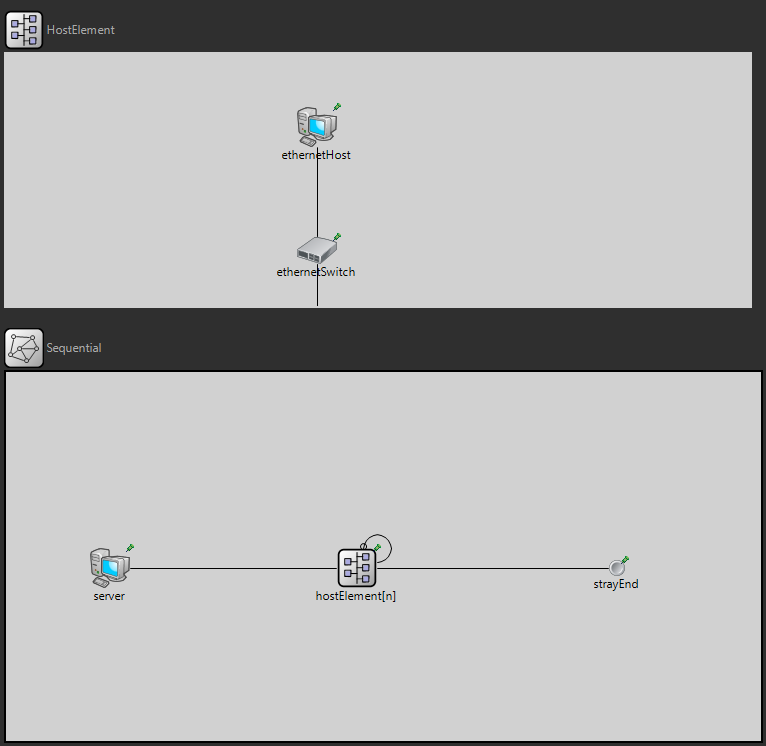
\includegraphics[width=1\textwidth]{sequential_network/sequential_layout.png}
    \caption{Sestava zaporedno vezanega omrežja}
    \label{g05:fig:sequential-layout}
\end{figure}

\subsubsection{Rezultati simulacij}

\begin{figure}[H]
    \centering
    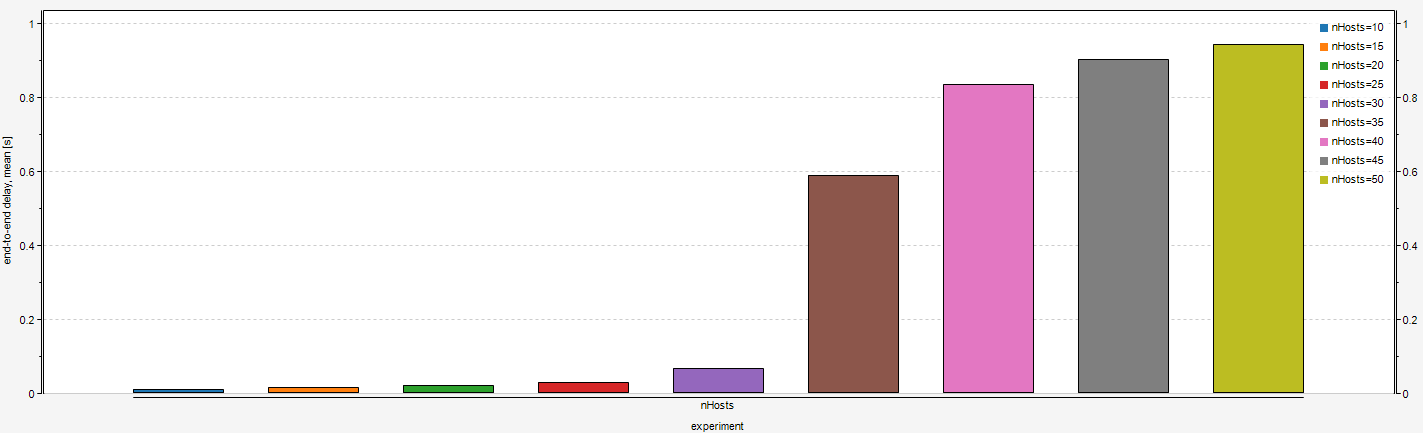
\includegraphics[width=1\textwidth]{sequential_network/sequential_nHosts.png}
    \caption{Vpliv števila verižnih členov}
    \label{g05:fig:sequential-nHosts}
\end{figure}

Kot je razvidno iz slike \ref{g05:fig:sequential-nHosts}, se čas prenosa podatkov povečuje z večanjem števila verižnih členov. To je posledica večje zakasnitve, ki se kopiči z vsakim dodatnim členom.
Lahko rečemo da je omrežje do 30 verižnih členov podobremnjeno, 35, mogoče celo 40 členov lahko klasificiramo kot normalno obremenitev. Karkoli več od 45 členov pa povzroči preobremenitev. Kot je iz grafa razvidno se čas potovanja ustali pri približno 1s, kar pomeni, da je presežek paketov zavržen zaradi preobremenitve.

\begin{figure}[H]
    \centering
    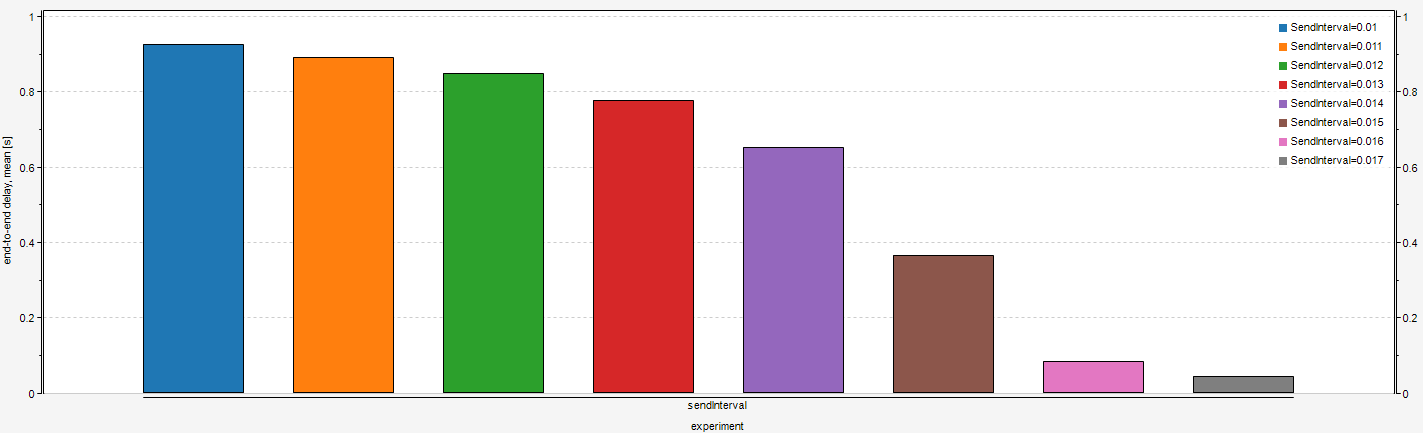
\includegraphics[width=1\textwidth]{sequential_network/sequential_sendInterval.png}
    \caption{Vpliv hitrosti pošiljanja}
    \label{g05:fig:sequential-sendInterval}
\end{figure}

Iz slike \ref{g05:fig:sequential-sendInterval} lahko razberemo, da je čas prenosa podatkov obratno sorazmeren s hitrostjo prenosa. Ko se pakete pošilja hitreje pride do prezasedenosti in daljše čakalne vrste, kar poveča skupno zamudo. Nasprotno, ko se interval pošiljanja poveča (paketi se pošiljajo redkeje), se prometna obremenitev zmanjša in sorazmerno s tem tudi čas potovanja paketa zmanjša.

\begin{figure}[H]
    \centering
    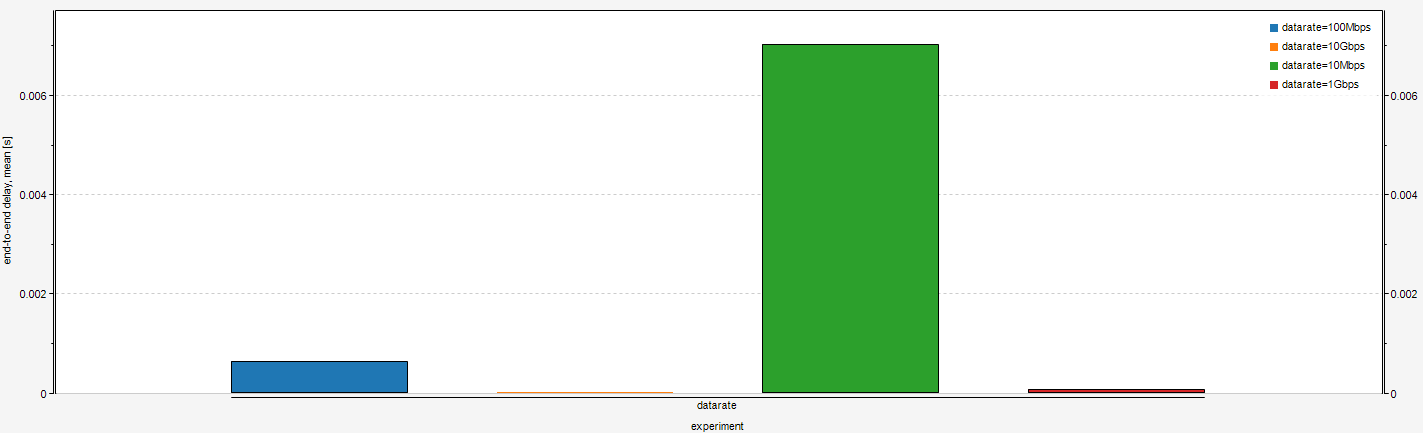
\includegraphics[width=1\textwidth]{sequential_network/sequential_datarate.png}
    \caption{Vpliv hitrosti prenosnih medijev}
    \label{g05:fig:sequential-datarate}
\end{figure}

Kot vidimo, povezava 10 Mb/s izstopa z največjim vplivom na hitrost omrežja, medtem ko povezave 1 Gb/s in 10 Gb/s ohranjajo skoraj zanemarljivo zakasnitev. To je intuitivno smiselno: počasnejše povezave porabijo več časa za prenos paketov, kar drastično poveča zakasnitev, medtem ko lahko hitrejše povezave prenesejo enako količino podatkov v veliko krajšem času. Kljub temu, pa se moramo zavedati, da v tem konkretnem primeru, kjer omrežje ni preobremenjeno govorimo o razlikah v milisekundah, kar je za uporabnika neopazno.

\begin{figure}[H]
    \centering
    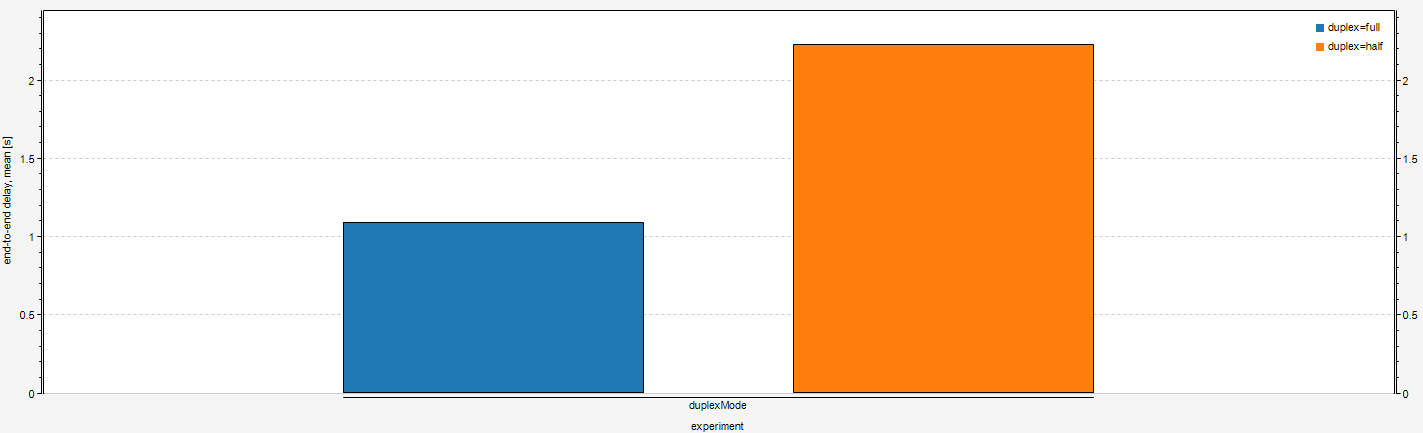
\includegraphics[width=1\textwidth]{sequential_network/sequential_duplex.png}
    \caption{Vpliv dvosmerne komunikacije}
    \label{g05:fig:sequential-duplexMode}
\end{figure}

Pri half-duplex načinu si oddajne in sprejemne operacije delijo isti kanal, kar lahko privede do kolizij in, v primeru da je CSMA vključen, povzroči zamude zaradi čakanja na prostost kanala. Zato je čas dostave pri half-duplexu opazno višji. V full-duplex načinu lahko vozlišča hkrati pošiljajo in prejemajo, s čimer se izognejo trkom in pomanjšajo čas dostave, saj ni treba čakati na nezasedenost prenosnega medija toliko kot pri half-duplexu. To ne pomeni, da do kolizij ne prihaja, pomeni le, da ne pride kolizij, ko se pošilja iz dveh koncev. Seveda, če si prenosni medij deli več naprav še vedno obstaja verjetnost kolizij ob istočasnem pošiljanju.

\begin{figure}[H]
    \centering
    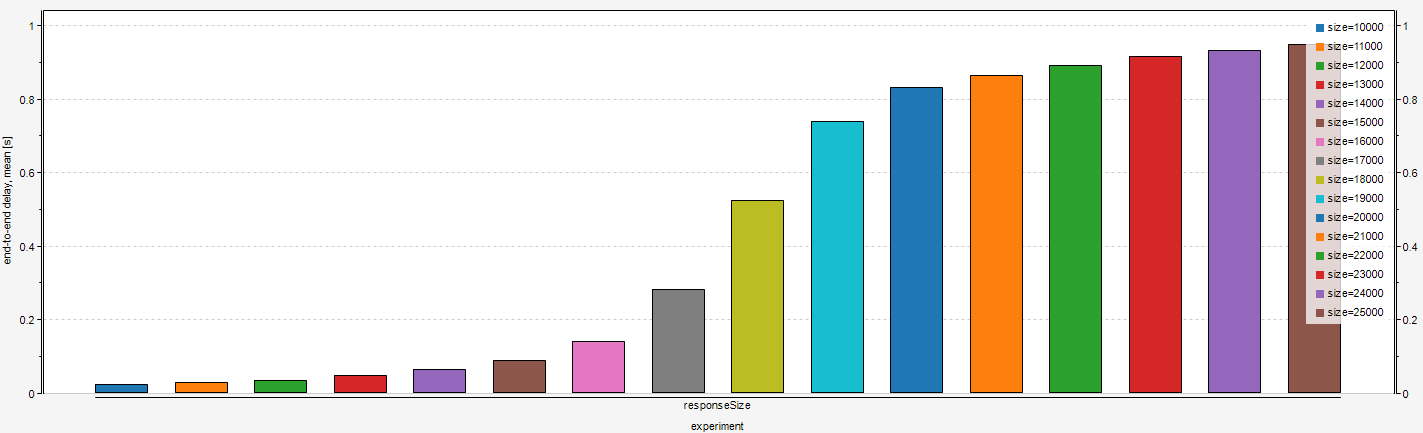
\includegraphics[width=1\textwidth]{sequential_network/sequential_responseSize.png}
    \caption{Vpliv velikosti odziva}
    \label{g05:fig:sequential-responseSize}
\end{figure}

Ko se velikost odziva poveča, se čas prenosa podatkov znatno poveča. Z drugimi besedami, prenos večih paketov povzroči kopičenje paketov v vrstah, tako da čas dostave vztrajno narašča z večjimi velikostmi odzivov. Manjša sporočila na levi strani grafikona povzročajo neopazno kopičenje. Okoli velikosti 17000B pa se vpliv na hitrost omrežja začne opazno povečevati.

\subsection{Mešano omrežje}

\subsubsection{Opis omrežja}

Mešano omrežje združuje tri različne Ethernet topologije, ki so vse medsebojno povezane preko skupnega vodila, sestavljenega iz več \texttt{WireJunction} modulov. Na to skupno vodilo se priključijo:
\begin{enumerate}
    \item \textbf{Zvezda z zvezdiščem:} Modul \texttt{EthernetHub} je povezan z več \texttt{EthernetHost} vozlišči.
    \item \textbf{Zvezda s stikalom:} Modul \texttt{EthernetSwitch} je prav tako povezan z več \texttt{EthernetHost} vozlišči.
    \item \textbf{Zaporedna veriga (\texttt{HostElement}):} V tej verigi je $n$ sestavljenih modulov \texttt{HostElement}, pri čemer je prvi člen povezan na vodilo, zadnji pa se konča pri \texttt{WireJunction} (imenovan \texttt{strayEnd}). Vsak \texttt{HostElement} združuje \texttt{EthernetHost} in \texttt{EthernetSwitch}, ki sta serijsko povezana. Pravzaprav gre za podobno strukturo kot v prejšnjem primeru, le da je tokrat prvi \texttt{HostElement} povezan na vodilo.
\end{enumerate}

\noindent
Tako nastane \textbf{mešano omrežje}, v katerem se vsa tri podomrežja priključijo na skupno vodilo ter skupaj tvorijo eno samo Ethernet omrežje.

\begin{figure}[H]
    \centering
    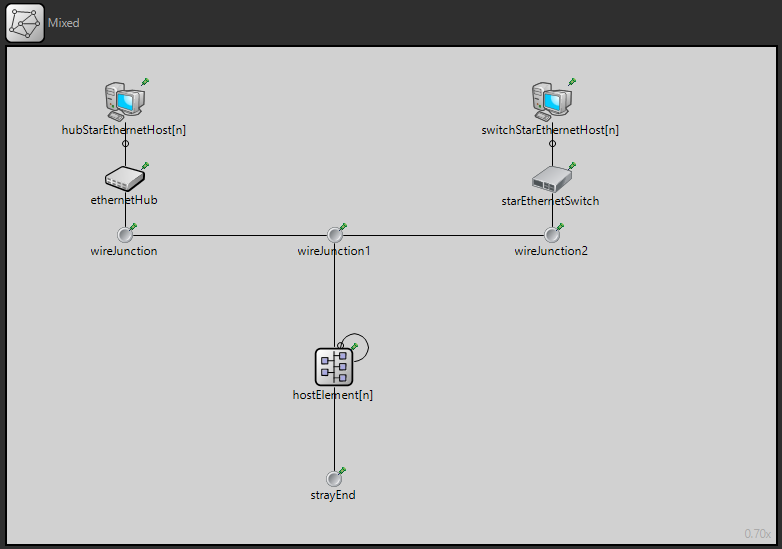
\includegraphics[width=1\textwidth]{mixed_network/mixed_layout.png}
    \caption{Sestava mešanega omrežja}
    \label{g05:fig:mixed-layout}
\end{figure}

\subsubsection{Rezultati simulacij}

\begin{figure}[H]
    \centering
    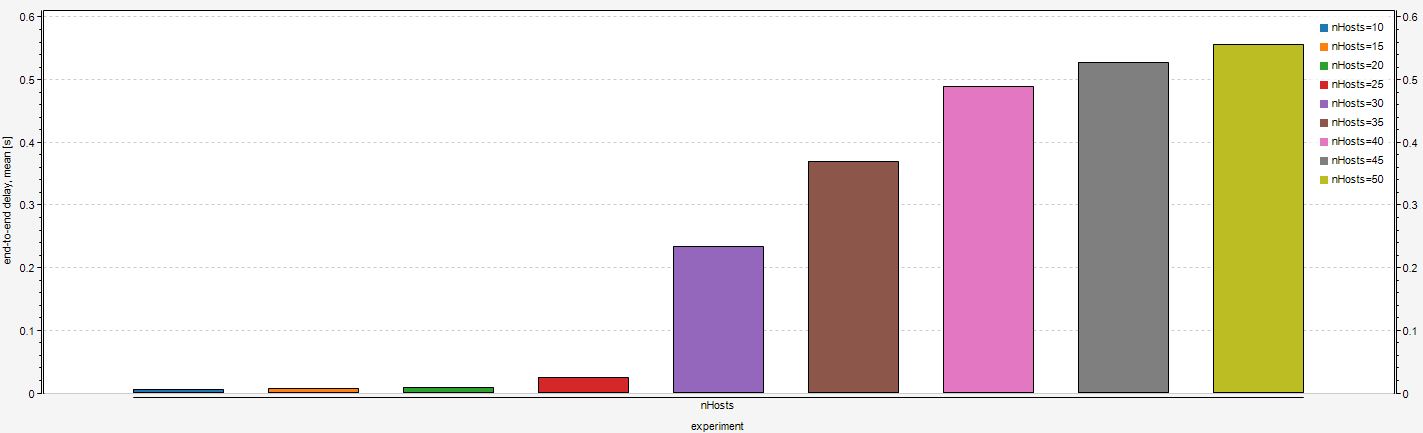
\includegraphics[width=1\textwidth]{mixed_network/mixed_nHosts.png}
    \caption{Vpliv števila verižnih členov}
    \label{g05:fig:mixed-nHosts}
\end{figure}

Kot je razvidno iz slike \ref{g05:fig:mixed-nHosts}, se čas prenosa podatkov povečuje z večanjem števila \texttt{EthernetHost}-ov na vsakem podomrežju.
Glede na grafikon lahko sklepamo, da je omrežje s 30 \texttt{EthernetHost}-i na podomrežje, podobremnjeno, 35 in 40 \texttt{EthernetHost}-ov predstavlja normalno obremenitev. Karkoli več od 45 \texttt{EthernetHost}-ov na podomrežje pa lahko klasificiramo kot preobremenitev za mešano omrežje. Kot lahko vidimo, se čas potovanja ustali pri približno 0,55s. Večja obremenitev samo povroči več zavrženih paketov.

\begin{figure}[H]
    \centering
    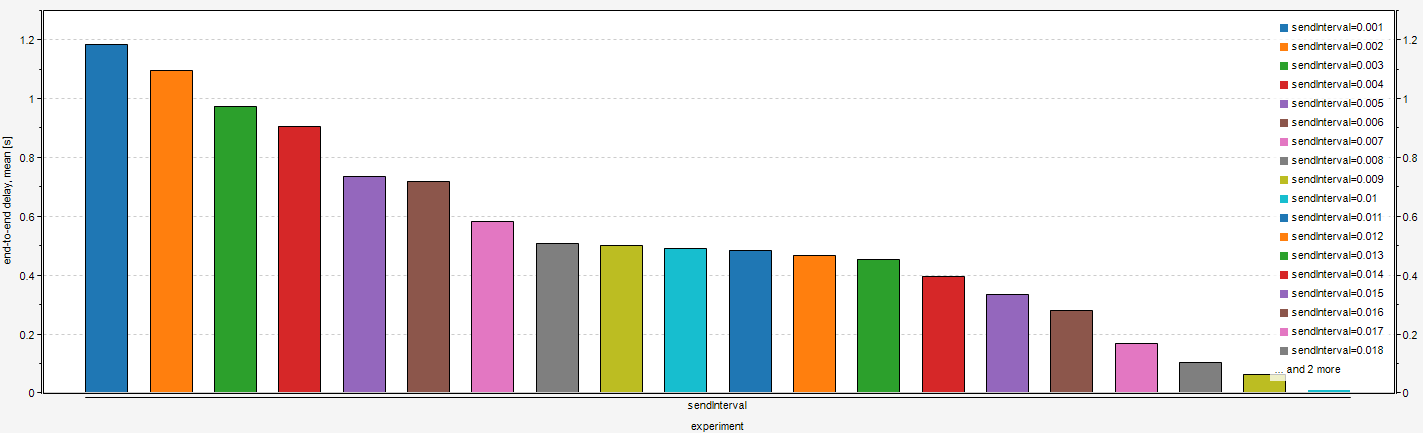
\includegraphics[width=1\textwidth]{mixed_network/mixed_sendInterval.png}
    \caption{Vpliv hitrosti pošiljanja}
    \label{g05:fig:mixed-sendInterval}
\end{figure}

Iz slike \ref{g05:fig:mixed-sendInterval} lahko razberemo, da je čas prenosa podatkov obratno sorazmeren s hitrostjo prenosa, ravno tako kot pri zaporedno vezanem omrežju. Ko je interval pošiljanja manjši pride do nasičenosti vrst, kar poveča čas potovanja paketa. Logično, ko se interval pošiljanja poveča, se obremenitev zmanjša in zamuda se znatno izboljša.

\begin{figure}[H]
    \centering
    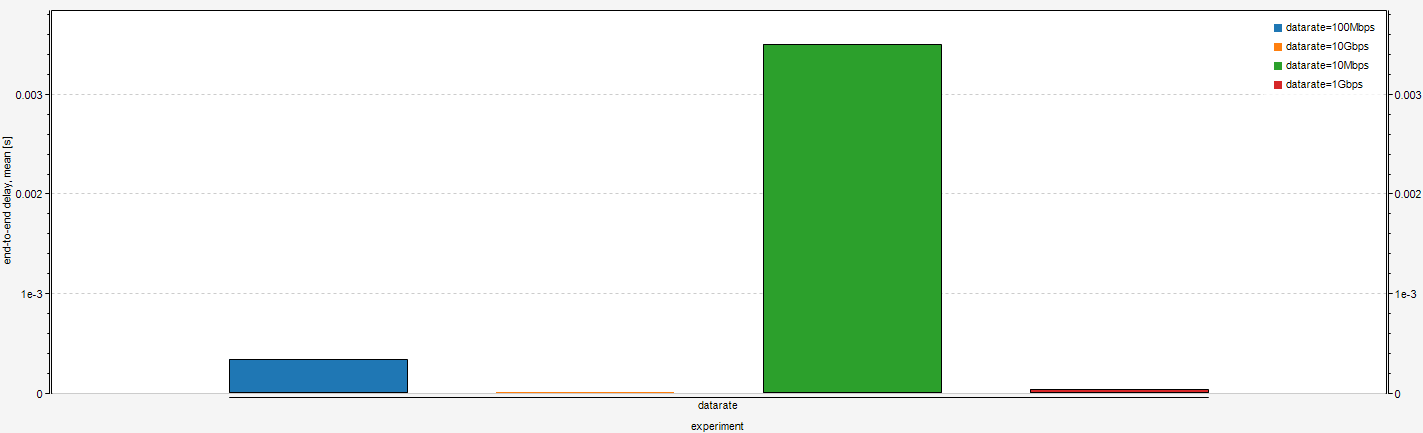
\includegraphics[width=1\textwidth]{mixed_network/mixed_datarate.png}
    \caption{Vpliv hitrosti prenosnih medijev}
    \label{g05:fig:mixed-datarate}
\end{figure}

Kot vidimo, ima povezava 10 Mb/s največji vpliv na hitrost omrežja, medtem ko povezave je zamuda pri 1 Gb/s in 10 Gb/s praktično zanemarljiva. Počasnejše povezave porabijo več časa za prenos podatkov, kar v zameno poveča zamudo, medtem ko lahko hitrejše povezave prenesejo enako količino paketov v občutno krajšem času. Sicer pa v tem primeru, kjer omrežje ni preobremenjeno govorimo o razlikah v milisekundah, kar je za uporabnika neobčutno.

\begin{figure}[H]
    \centering
    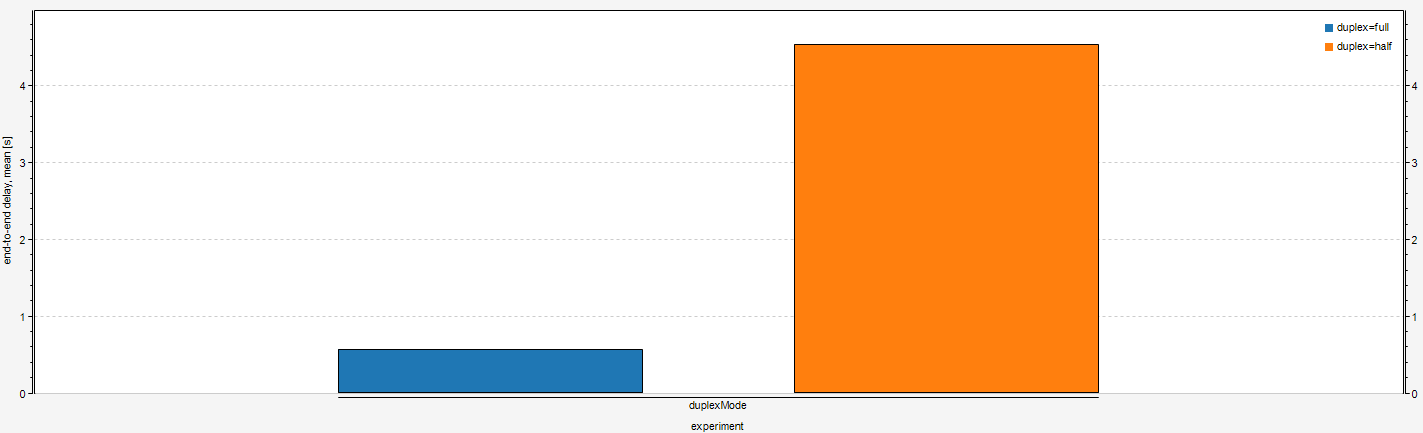
\includegraphics[width=1\textwidth]{mixed_network/mixed_duplex.png}
    \caption{Vpliv dvosmerne komunikacije}
    \label{g05:fig:mixed-duplexMode}
\end{figure}

Pri half-duplex načinu je na istem kanalu možna le enosmerna komunikacija, kar lahko privede do kolizij in zakasnitev zaradi čakanja na prostost kanala (v primeru, da je CSMA vključen). Zato je čas potovanja paketa pri half-duplexu opazno višji. V full-duplex načinu je vklučena dvosmerna komunikacija, s čimer se izognejo trkom in pomanjšajo čas potovanja paketa, saj ni treba čakati na nezasedenost prenosnega medija toliko kot pri half-duplexu. To ne pomeni, da do kolizij ne prihaja. Pomeni le, da ne pride do kolizij, ko se pošilja iz dveh koncev. Seveda, če si prenosni medij deli več naprav še vedno obstaja verjetnost kolizij.

\begin{figure}[H]
    \centering
    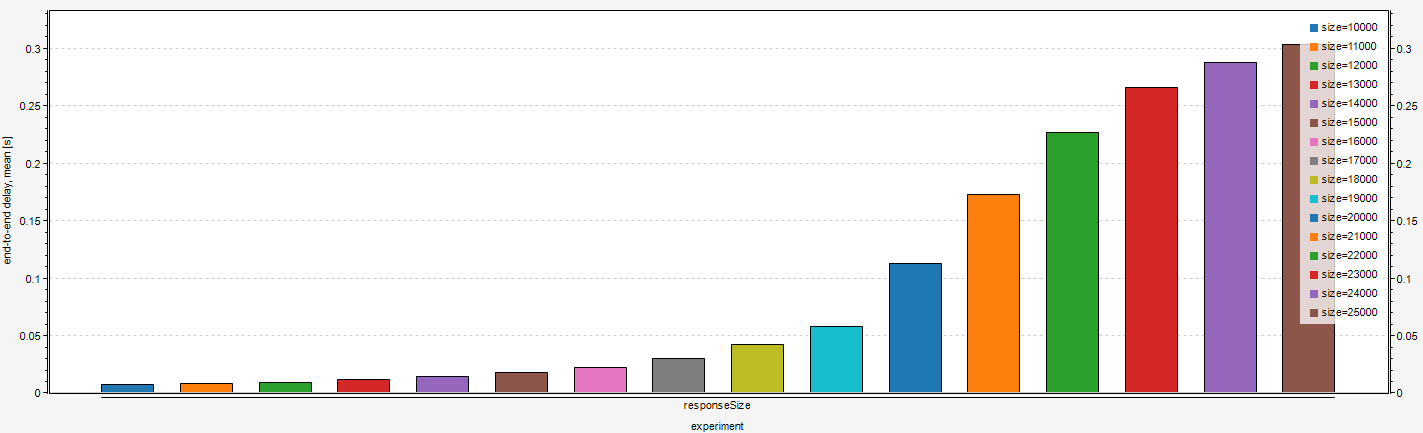
\includegraphics[width=1\textwidth]{mixed_network/mixed_responseSize.png}
    \caption{Vpliv velikosti odziva}
    \label{g05:fig:mixed-responseSize}
\end{figure}

Ko se velikost odziva poveča, se čas prenosa podatkov občutno poveča. Drugače povedano, prenos večih paketov povzroči napolnjenje vrst, tako da čas dostave sorazmerno narašča z večjimi velikostmi odzivov. Na levi strani grafa lahko vidimo majhne velikosti odzivov, ki očitno povzročajo neopazno kopičenje. Okoli velikosti 17000B pa se vpliv na hitrost omrežja začne hitro povečevati.

\section{Zanimiva opažanja}

Med simuliranjem in analiziranjem izbranih omrežji smo opazili tudi nekaj zanimivih primerov, za katere nismo pričakovali, da se bodo zgodili. Nismo prepričani, če so to dejanske lastnosti omrežij, ki jih modeliramo, ali pa so posledica implementacije v ogrodju $INET$ oziroma samega programa $OMNeT++$.

\paragraph{}

Ena izmed teh je recimo obnašanje zakasnitve paketov, v odvisnosti of kapacitete čakalnih vrst stikal. Pričakovali bi, da se bo zakasnitev zmanjševala z večanjem kapacitete čakalnih vrst. Rezultati tega ne namigujejo. Simulacije smo seveda pognali večkrat na razširjeni dvojni zvezdi in binarnemu ethernet drevesu in nismo dobili razultatih, ki bi pokazale intuitivno povezavo med zakasnitvijo paketov in kapaciteto čakalnih vrst. 

\begin{figure}[H]
    \centering
    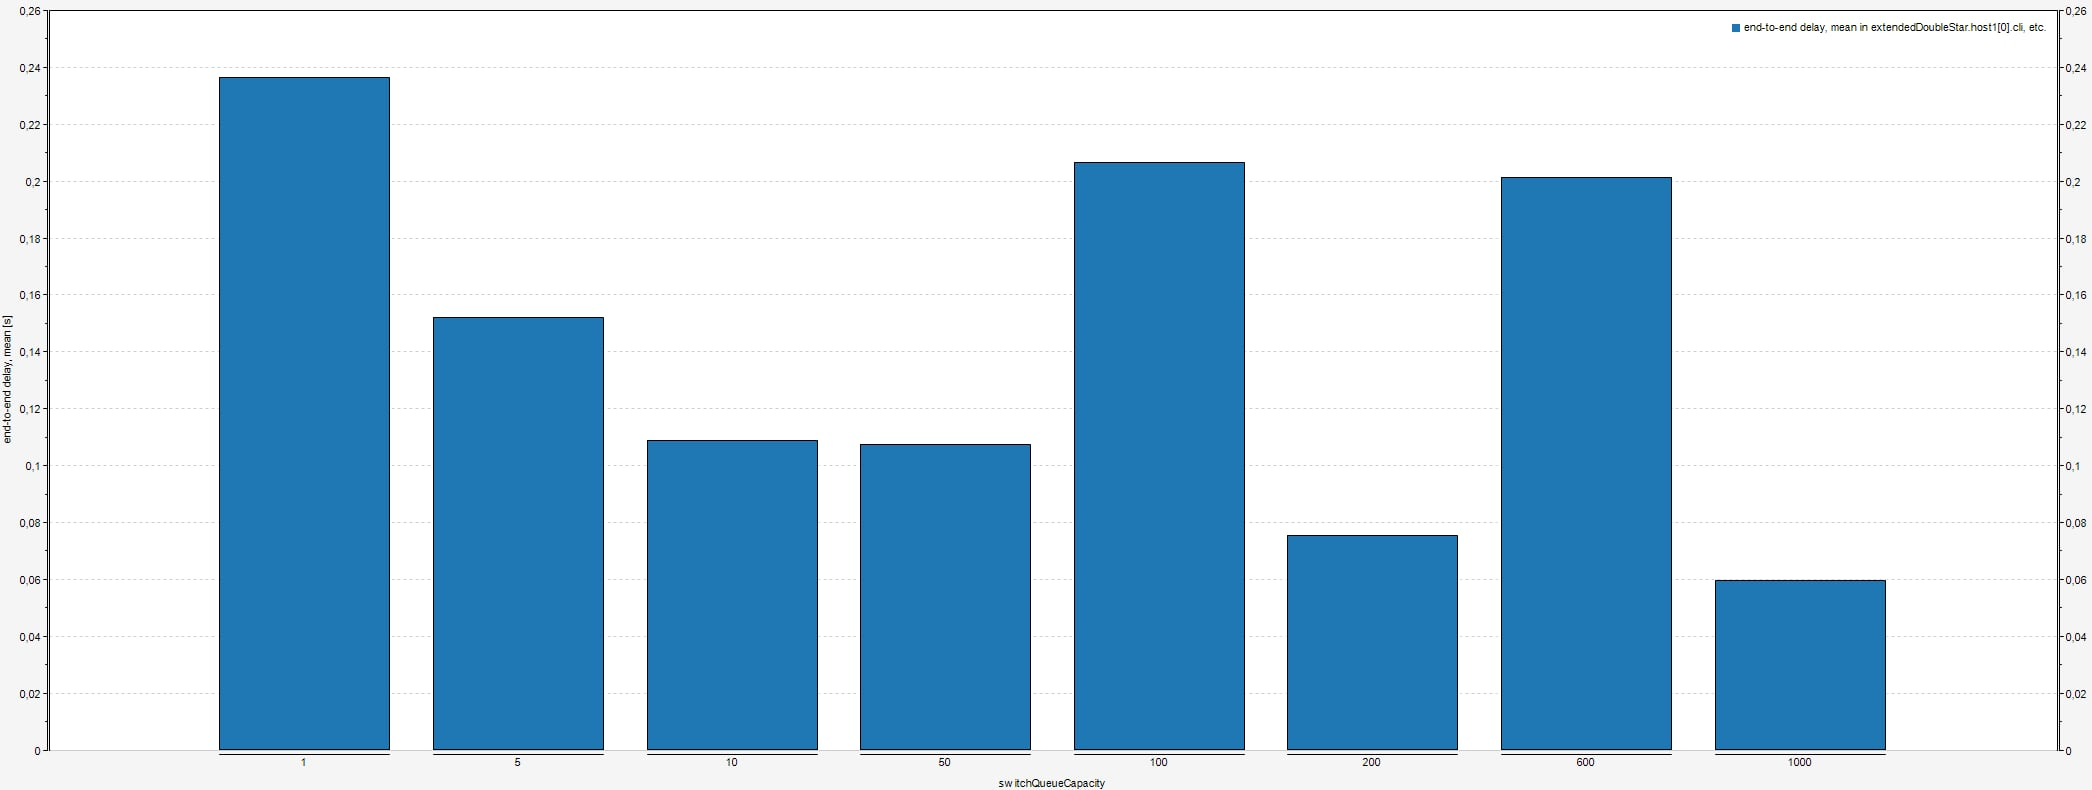
\includegraphics[width=1\textwidth]{extended-double-star/switch-queue-length-end-to-end-delay.png}
    \caption{Zakasnitev paketov v odvisnosti od kapacitete čakalnih vrst stikal v omrežju razširjene dvojne zvezde}
    \label{fig:switch-queue-cap-end-to-end-delay-double-star}
\end{figure}

\begin{figure}[H]
    \centering
    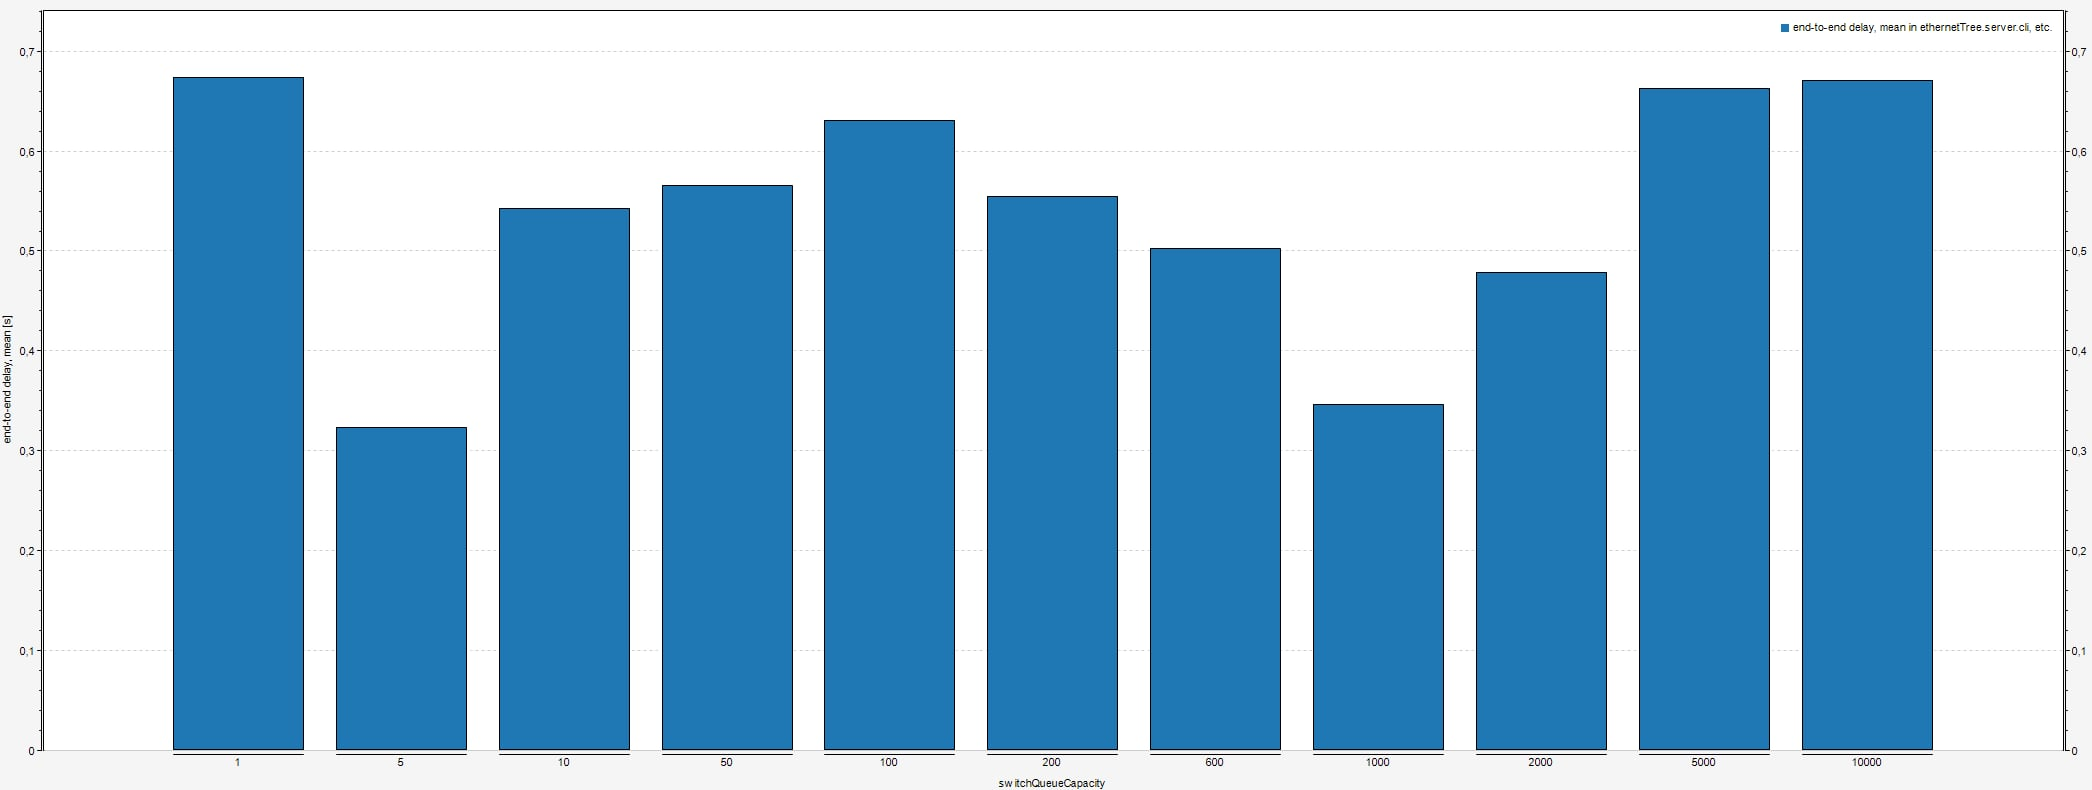
\includegraphics[width=1\textwidth]{binary-tree/switch-queue-length-end-to-end-delay.jpg}
    \caption{Zakasnitev paketov v odvisnosti od kapacitete čakalnih vrst stikal v omrežju binarnega ethernet drevesa}
    \label{fig:switch-queue-cap-end-to-end-delay-binary-tree}
\end{figure}

Opazili smo tudi razultat, ki se nam je sprva zdel izjemno sumljiv in neintuitiven. Ko smo omrežje opazovali z vklopljenim CSMA/CD načinom, smo v rezulzatih videli veliko kolizij. Ko pa smo isto omrežje opazovali pod istimi pogoji z izključenim CSMA/CD načinom, smo opazili, da kolizij ni bilo. To se nam je zdelo zelo čudno, saj smo pričakovali ravno nasprotno. Ugotovili smo, da je to posledica implementacije v ogrodju $INET$. Ko je CSMA/CD način izključen, se kolizije sploh ne beležijo.

\begin{figure}[H]
    \centering
    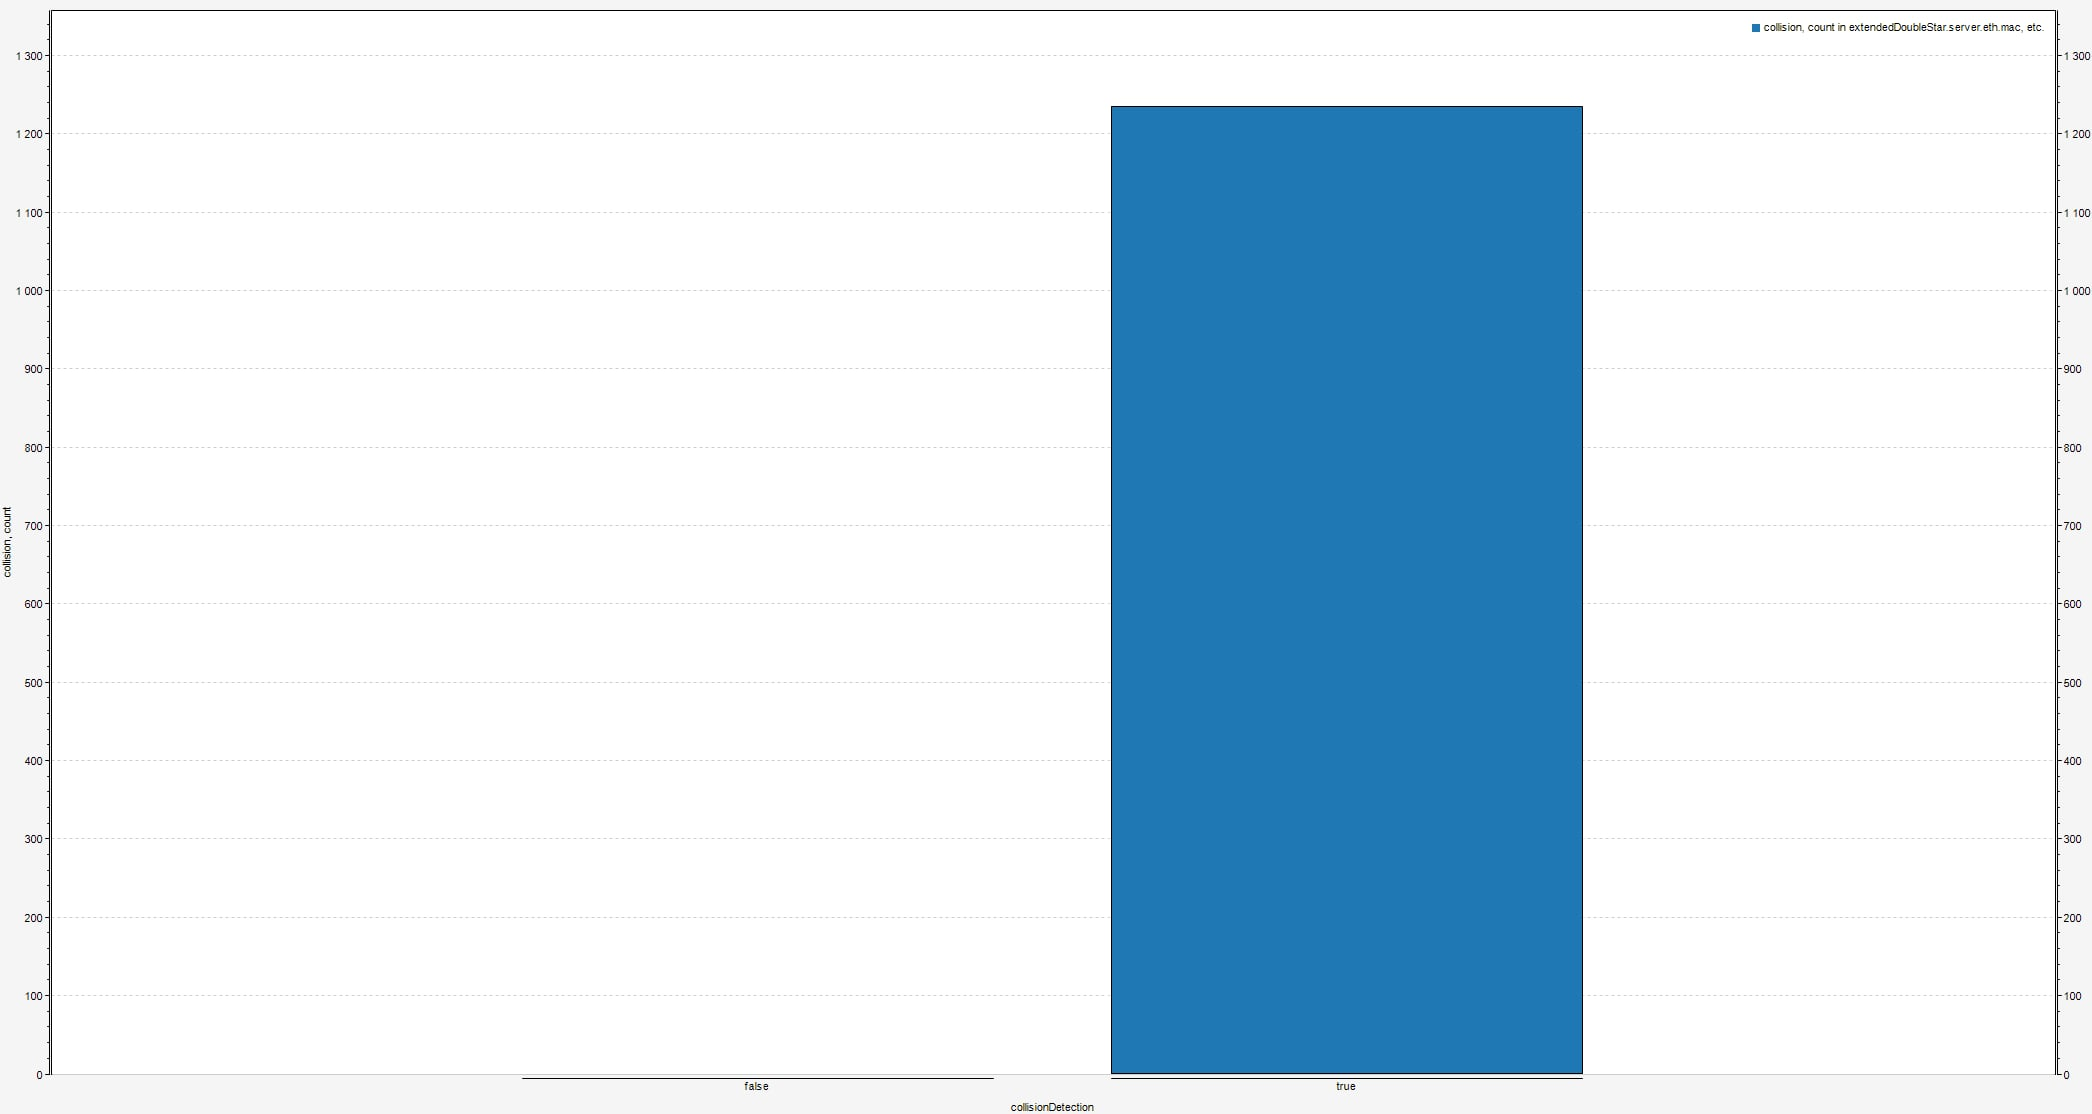
\includegraphics[width=1\textwidth]{extended-double-star/csma-collisions.jpg}
    \caption{Število zaznanih kolizij pri vključenem in izključenem CSMA/CD načinu v omrežju razširjene dvojne zvezde}
    \label{fig:csma-cd-collisions-binary-tree}
\end{figure}

\section{Sklepi in zaključek}

Skozi vsa omrežja je bilo glavno opažanje to, da je meja med normalnim in nenormalim delovanjem omrežja velikokrat zelo tanka in zelo očitna. Praktično za vsak zvezen parameter, za katerega smo opazovali vpliv na delovanje omrežja, smo opazili, da je pri neki vrednosti omrežje izjemno občutljivo na majhne spremembe tega parametra. Vsi parametri, ki smo jih opazovali so imeli občuten vpliv na zakasnitev paketov. Večina rezulzazov se nam je zdela intuitivnih, nekaj pa jih je bilo tudi zelo presenetljivih, ki so pokazale tudi meje ogrodja $INET$ in programa $OMNeT++$.
\paragraph{}
Ugotovili smo tudi, da so nasplošno ethernet omrežja izjemno hitra in da jih moramo izjemno obremeniti, če želimo videti kakšne resne zakasnitve. Velik vpliv na normalno delovanje imajo tudi kolizije, ki se pojavijo, ko je omrežje preobremenjeno, ali pa če je preveč skupnih vodil. Pri tem smo opazili, da nam kombinacija stikal in uporaba CSMA/CD načina omogoča, da vpliv kolizij nevtraliziramo.
